% !TEX jobname=projet_epidemio_bigarre

\documentclass[11pt]{article}
\usepackage[french]{babel}
\usepackage[top=3.5cm,bottom=3cm, right=3cm,left=3cm]{geometry}
\usepackage{amsmath}
\usepackage{amsfonts}
\usepackage{graphicx}
\usepackage{subcaption}
\usepackage{url}

\newcommand{\deriv}{\texttt{d}}
\newcommand{\dt}[1]{\frac{\deriv #1}{\deriv t}}
\newcommand{\ssi}{\Longleftrightarrow}

\author{Célestin \bsc{BIGARR\'E}}
\title{Projet d'\'epidemiologie}


\begin{document}
\maketitle

\section{Exercice 1}
\begin{figure}
	\centering
	\includegraphics{shema ex 1.eps}
	\caption{Sch\'ema du mod\`ele de la rage dans une population de renards}
	\label{fig:schema ex 1}
\end{figure}
On cherche dans cet excercice modeliser une \'epidemie de rage dans une population de renards. On propose le mod\`ele sch\'ematis\'e \`a la Figure \ref{fig:schema ex 1}. Le syst\`eme d'\'equations associ\'e est :
\[
\left\{
	\begin{aligned}
		\dt S &= a (S+E+I) -b S - \gamma (S+E+I)S - \beta I S\\
		\dt E &= \beta IS - b E - \gamma (S+E+I)E - \sigma E\\
		\dt I &=  \sigma E - b I - \gamma (S+E+I)I - \alpha I 
	\end{aligned}\right.
\]

\subsection{\'Etude de l'\'equilibre sain}

On cherche maintenant un \'etat d'\'equilibre non nul $(\tilde S, \tilde E, \tilde I)$ sans maladie (DFE). C'est-\`a-dire v\'erifiant,
\[
\left\{
	\begin{aligned}
		\dt S (\tilde S) &= 0\\
		\tilde E &= 0\\
		\tilde I &= 0
	\end{aligned}\right.
\]

On obtient pour ce syst\`eme l'\'equation logistique bien connue, 
\begin{align*}
	\dt S (\tilde S) &= (a-b) S - \gamma S^2\\
	&= (a-b) S (1 - \frac{\gamma}{a-b})
\end{align*}


Le seul \'equilibre non nul pour cette \'equation est, $\tilde S = \frac{a-b}{\gamma} = K$. Le seul DFE pour le syst\`eme \'etudi\'e est donc $(K, 0, 0)$.

\paragraph{} Connaissant cet \'equilibre sain, on peut calculer le taux de reproduction de base, $R0$. 

\paragraph{}
Commencons par chercher une matrice $M_1$ telle que, 
\[
\dt S = M_1(S, E, I)  \cdot 
	\begin{pmatrix}
		S- K\\
		E \\
		I \\
	\end{pmatrix}.
\]
 Or, on a, 

 \begin{align*}
	 dt S &= (a-b)S - \gamma S (S+E+I) - \beta I S + a E + aI \\
	      &= (a - b- \gamma N - \gamma K)(S-K) + \frac{a-b}{\gamma} \left(a-b- \gamma N (K + E + I) \right) - \beta SI + a (E +I)\\
	      &= -\gamma N (S-K) + bE + (b- \beta S) I 
\end{align*}

D'o\`u, $M_1 = \begin{pmatrix} -\gamma N & b  & b - \beta S \end{pmatrix}$.

\paragraph{} On pose de plus $M_1 = [M_{11}\quad M_{12}]$ avec :
\[
M_{11} = (-\gamma N) \text{ et } M_{12} = \begin{pmatrix}b & b - \beta S \end{pmatrix}
\]

On cherche aussi $M_{22}$ telle que,
\[
\begin{pmatrix}\dt E \\ \dt I\end{pmatrix}= M_{22}(S,E,I) \cdot \begin{pmatrix}S\\I\end{pmatrix}
\]

De mani\`ere \'evidente, $M_{22} = \begin{pmatrix}-b -\sigma-\gamma(S+E+I) & \beta S\\ \sigma & -b-\alpha-\gamma(S+E+I)\end{pmatrix}$

\paragraph{}
Ainsi la jacobienne du syst\`eme au  point $(K,0,0)$ s'\'ecrit, 
\begin{align*}
	J(K,0,0) &= \begin{bmatrix}
		M_{11}(K,0,0) & M_{12}(K,0,0) \\ 0 & M_{22}(K,0,0)
	\end{bmatrix}\\
	&= \begin{pmatrix}
	-\gamma K & b & b\\
	0 & -b-\sigma - \gamma K  & \beta K\\
	0&  \sigma & -b - \alpha - \gamma K
	\end{pmatrix}
\end{align*}
Mais aussi, 
\begin{align*}
	J(K,0,0) &= 
		\begin{bmatrix}
			M_{11}(K,0,0) & M_{12}(K,0,0) \\ 0 & 
			\begin{pmatrix}
				-b-\sigma - \gamma K  & 0\\
				\sigma & -b - \alpha - \gamma K
			\end{pmatrix}
		\end{bmatrix} + 
		\begin{bmatrix}
			0 & 0 \\ 0 & 
			\begin{pmatrix}
				0 & \beta K\\
				0 & 0
			\end{pmatrix}
		\end{bmatrix}
\end{align*}

En posant, 
\[
	F = \begin{pmatrix}
				0 & \beta K\\
				0 & 0
			\end{pmatrix} \text{ et } V = \begin{pmatrix}
				-b-\sigma - \gamma K  & 0\\
				\sigma & -b - \alpha - \gamma K
			\end{pmatrix}
\]
et comme $F \geq 0$, $V$ est de Metzler et que $M_{22} =  F + V$, on a par d\'efinition :
\[
R_0 = \rho (-FV^{-1})
\] 


On a $\det V = (-b - \sigma -\gamma K)(-b-\alpha - \gamma K)$  donc,
\[
V^{-1} = \begin{pmatrix}
	\frac{1}{- b- \sigma - \gamma K} & 0 \\ 
	\frac{\sigma}{(-b - \sigma -\gamma K)(-b-\alpha - \gamma K)} & \frac{\beta K}{-b -\alpha - \gamma K}
\end{pmatrix}
\]
et par suite, 
\[
-F V^{-1} = 
\begin{pmatrix}
	\frac{-\beta K \sigma }{(-b - \sigma -\gamma K)(-b-\alpha - \gamma K)} & \frac{\beta K}{-b -\alpha - \gamma K} \\ 
	0 & 0
\end{pmatrix}
\]
D'o\`u le polyn\^ome caracteristique de $-FV^{-1}$ est $-\lambda \left(\frac{-\beta K \sigma }{(-b - \sigma -\gamma K)(-b-\alpha - \gamma K)} - \lambda \right)$ donc $\text{sp} (-FV^{-1}) = \{0, \frac{-\beta K \sigma }{(-b - \sigma -\gamma K)(-b-\alpha - \gamma K)} \}$ et 
\begin{align*}
 R_0 &=\frac{-\beta K \sigma }{(-b - \sigma -\gamma K)(-b-\alpha - \gamma K)}\\
 	 &= \frac{\beta (a-b) \sigma}{\gamma (a + \alpha)(a+\sigma)} \\
 	 &= K \frac{\beta \sigma}{(a + \alpha)(a+\sigma)}
 \end{align*}


\subsection{\'Equilibre end\'emique}
On s'int\'eresse mainenant \`a l'\'equilibre end\'emique. On cherche donc  $(\tilde S, \tilde E, \tilde I)$ avec $\tilde E \neq 0$ et $\tilde I \neq 0$ tel que :
\[
\left\{
	\begin{aligned}
		\dt S (\tilde S) &= 0\\
		\dt E (\tilde E) &= 0\\
		\dt I (\tilde I) &= 0
	\end{aligned}\right.
\] 

Pour trouver cet \'equilibre, on effectue le changement de variable suivant :

\[
\left\{
	\begin{aligned}
		\bar S &= \frac{S}{S+E+I}\\
		\bar I &= \frac{I}{S+E+I}\\
		N &= S+E+I
	\end{aligned}\right.
\] 

La formule des d\'eriv\'ees compos\'ees donne alors,
\begin{align*}
	&\left\{
	\begin{aligned}
		\dt{\bar S} &= \frac{N \dt S - S \dt N}{N^2}\\
		\dt{\bar E} &= \frac{N \dt E - E \dt N}{N^2}\\
		\dt{\bar I} &= \frac{N \dt I - I \dt N}{N^2}\\
		\dt N &= \dt S+ \dt E+ \dt I
	\end{aligned}\right.\\
	\ssi &\left\{
	\begin{aligned}
		\dt{\bar S} &= -b \bar S + a -\gamma N \bar S - \beta N \bar I \bar S - \bar S \left( (a -b)  - \gamma N -\alpha \bar I\right)\\
		\dt{\bar E} &= \beta N \bar I \bar S - (b + \sigma) \bar E -\gamma N \bar E - \bar E \left( (a -b)  - \gamma N -\alpha \bar I\right)\\
		\dt{\bar I} &= \sigma \bar E - (b+ \alpha) \bar I - \gamma N \bar I - \bar I \left( (a -b)  - \gamma N -\alpha \bar I\right)\\
		\dt N &= (a -b) N - \gamma N^2 -\alpha N \bar I
	\end{aligned}\right.\\
	\ssi &\left\{
	\begin{aligned}
		\dt{\bar S} &= a  - \left( a - \alpha \bar I + \beta N \bar I\right) \bar S\\
		\dt{\bar E} &= \beta N \bar I \bar S - (a + \sigma - \alpha \bar I) \bar E \\
		\dt{\bar I} &= \sigma \bar E - (a + \alpha- \alpha \bar I) \bar I\\
		\dt N &= (a -b) N - \gamma N^2 -\alpha N \bar I
	\end{aligned}\right.
\end{align*}

Le syst\`eme est entierement d\'ecrit par $\bar S, \bar E$ et $N$ car $\bar S+\bar E + \bar I = 1$. Trouver l'\'equilibre end\'emique revient \`a r\'esoudre,
\begin{align*}
	&\left\{
	\begin{aligned}
		\dt{\bar S} &= 0\\
		\dt{\bar I} &= 0\\
		\dt N &= 0
	\end{aligned}\right.\\
	\ssi &\left\{
	\begin{aligned}
		0 &= a  - \left( a - \alpha \bar I + \beta N \bar I\right) \bar S\\
		0 &= \sigma \bar E - (a + \alpha- \alpha \bar I) \bar I\\
		0 &= (a -b) N - \gamma N^2 -\alpha N \bar I
	\end{aligned}\right.
\end{align*}

On peut facilement exprimer $\bar N$ et $\bar S$ en fonction de $\bar I$, en effet 
\begin{align*}
	&\left\{
	\begin{aligned}
		\bar S &= \frac{a}  {a - \alpha \bar I + \beta N \bar I}\\
		0 &= \sigma (1- \bar S - bar I) - (a + \alpha- \alpha \bar I) \bar I\\
		0 &= a -b - \gamma N -\alpha \bar I
	\end{aligned}\right. \\
	\ssi& \left\{
	\begin{aligned}
		\bar S &= \frac{a}  {a - \alpha \bar I + \beta N \bar I}\\
		0 &= \sigma (1- \bar S - \bar I) - (a + \alpha- \alpha \bar I) \bar I\\
		N &= \frac{a -b  -\alpha \bar I}{\gamma}
	\end{aligned}\right. \\
	\ssi& \left\{
	\begin{aligned}
		\bar S &= \frac{a}  {a - \alpha \bar I + \beta N \bar I}\\
		\bar S &= 1 -\frac{(a + \sigma + \alpha - \alpha \bar I) \bar I}{\sigma}\\
		N &= \frac{a -b  -\alpha \bar I}{\gamma}
	\end{aligned}\right.
\end{align*}

\begin{figure}[ht]
\centering
	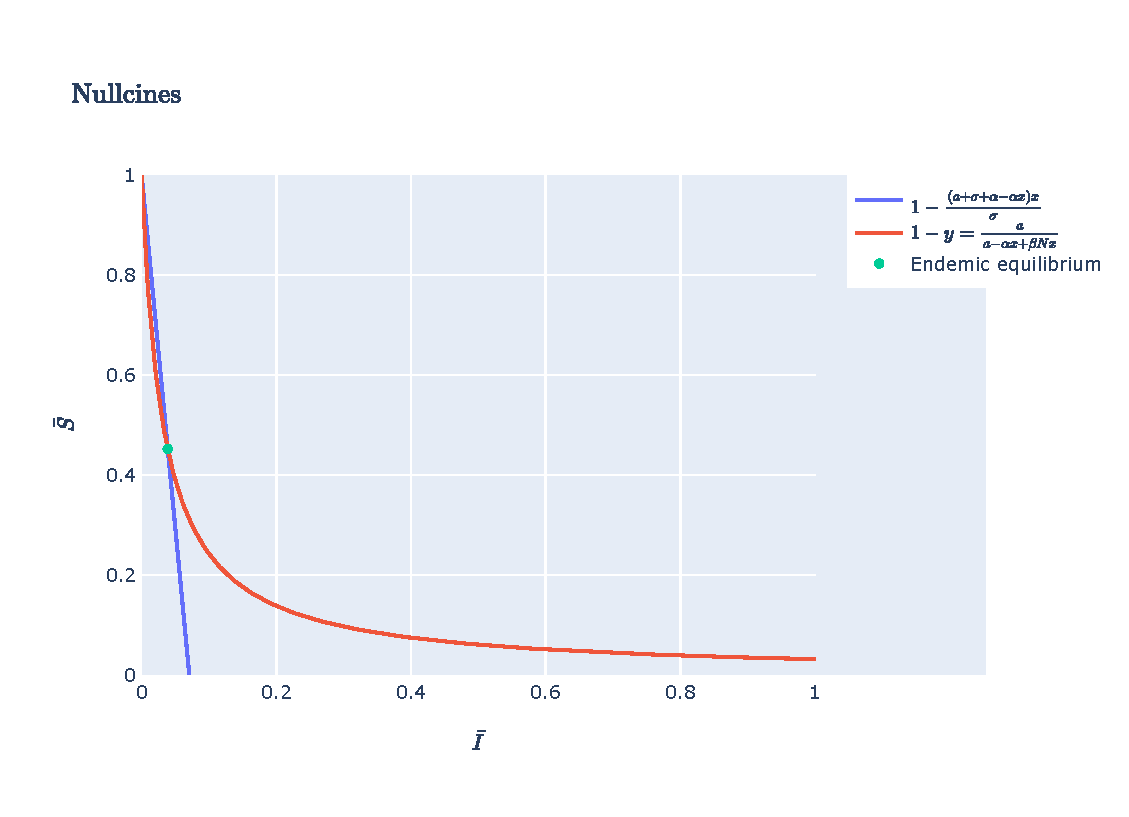
\includegraphics[width=0.8\linewidth]{../figures/nullclines.eps}
	\caption{\'Equilibre end\'emique de l'\'epidemie pour $b =0.5, a = 1, \sigma = \frac{1}{13}, \alpha = \frac{1}{73}, \beta = \frac{1}{79.69}$ et $\gamma = \frac{1}{5000}$}
\label{fig:equilibre endemique}
\end{figure}

Le syst\`eme ne peut malheureusement pas \^etre r\'esolu simplement (la combinaison des deux premi\`eres \'equations donne un polyn\^ome de degr\'e 4 en $\bar I$). Cette ecriture permet n\'eanmoins de determiner graphiquement ou num\'eriquement l'\'equilibre end\'emique. Il suffit pour cela de determiner si les courbes
\[
y = \frac{a}  {a - \alpha x + \beta N x} \quad \text{et} \\
y = 1 -\frac{(a + \sigma + \alpha - \alpha x) x}{\sigma}
\] 
se croisent sur le pav\'e $]0,1[\times ]0,1[$ (cf Figure \ref{fig:equilibre endemique}). Le point $(0,1)$ repr\'esentant le DFE est bien entendu toujours un point d'intersection. Lorsqu'on a determi\'e $\bar I$ on peut calculer $N$. Il ne reste plus ensuite qu'\`a reexprimer les variables du syt\`eme initial : $S = N \bar S, E = N (1-\bar S - \bar I)$ et $I = N \bar I$.



\subsection{Stabilit\'e de l'\'equilibre end\'emique}
Pour \'etudier la stabilit\'e de l'\'equilibre end\'emique, on explore num\'eriquement le portrait de phase de $E$  en fonction de $I$ et le comportement de la trajectoire par rapport \`a l'\'equilibre end\'emique. La Figure \ref{fig:endemic stability} propose ce portrait de phase pour deux jeux de param\`etres conduisant \` $R_0 > 1$.


\begin{figure}[hb]
\centering
\begin{subfigure}{0.49\textwidth}
  \centering
  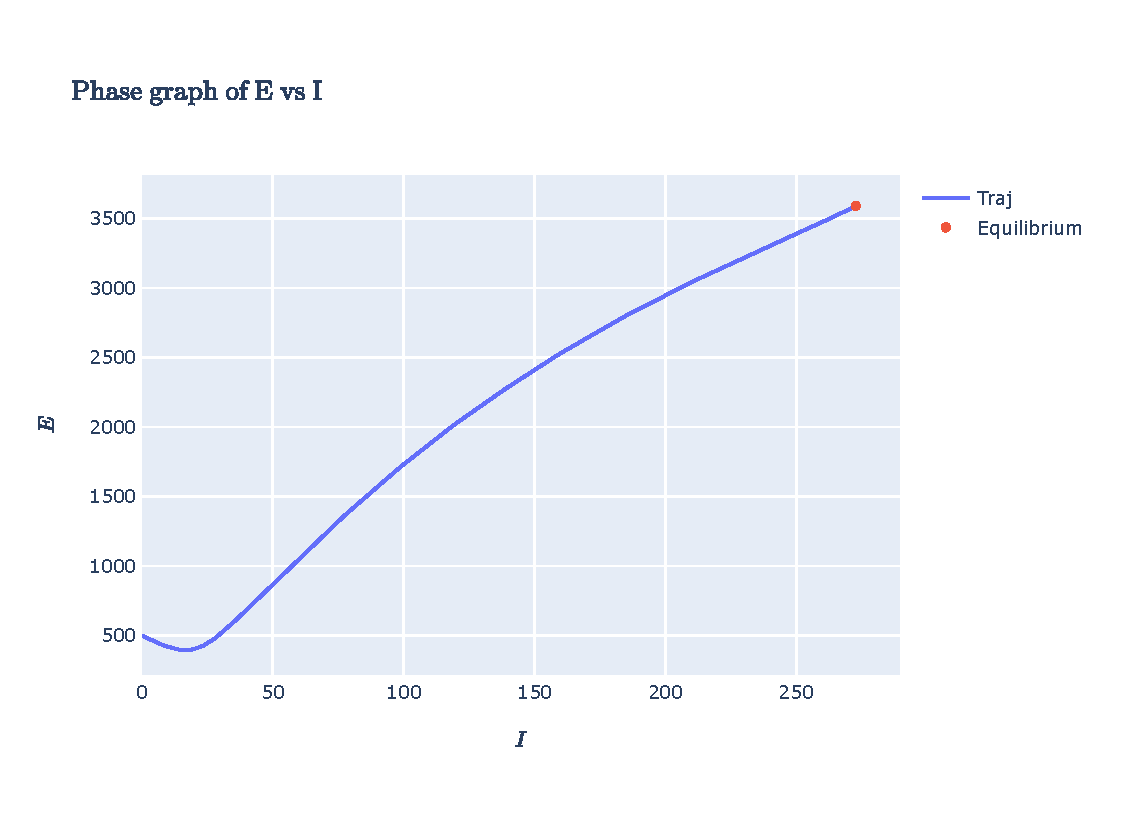
\includegraphics[width=\linewidth]{../figures/study_Endemic_stabillity_1.eps}  
  \caption{$b =0.5, a = 1, \sigma = \frac{1}{13}, \alpha = \frac{1}{73}, \\\beta = \frac{1}{79.69}$ et $\gamma = \frac{1}{10000}$ \\
  $S_0 = 1000, E_0 = 500, I_0 = 0$}
  \label{fig:endemic stability 1}
\end{subfigure}\
\begin{subfigure}{0.49\textwidth}
  \centering
  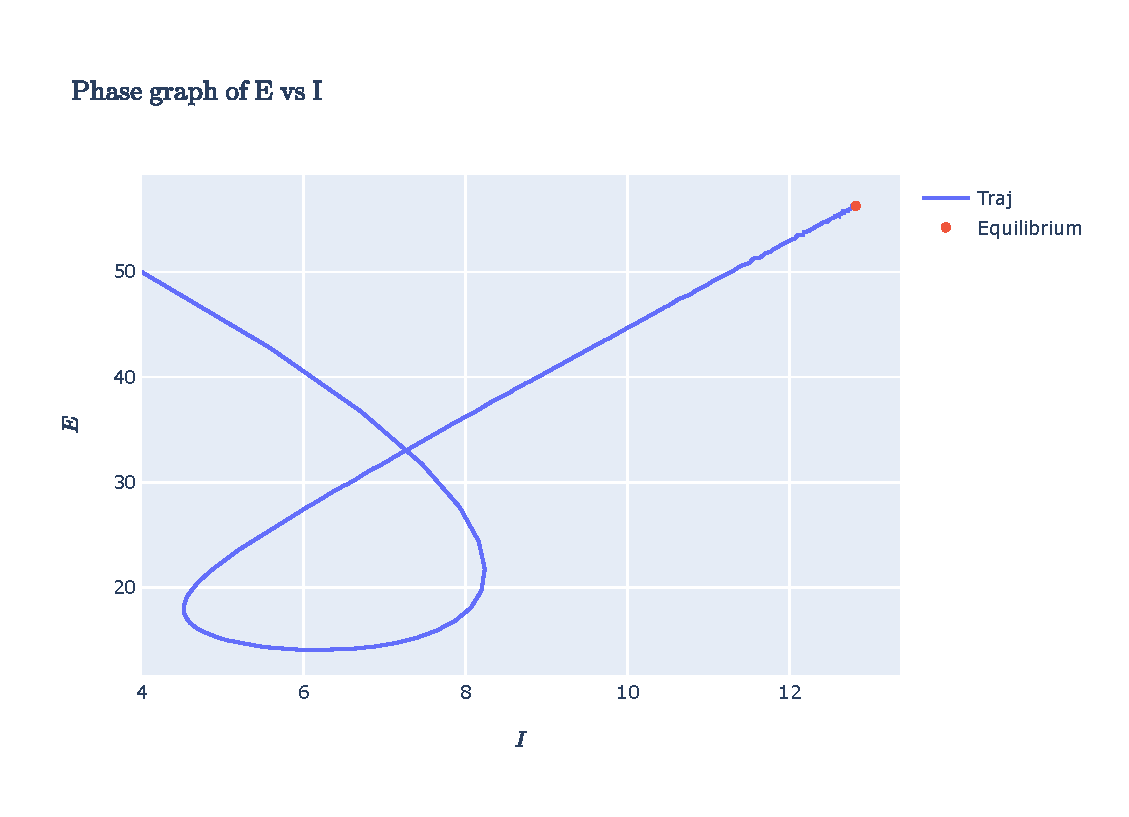
\includegraphics[width=\linewidth]{../figures/study_Endemic_stabillity_2.eps}
  \caption{$b =0.5, a = 1, \sigma = \frac{3}{13}, \alpha = \frac{1}{73}, \\\beta = \frac{1}{79.69}$ et $\gamma = \frac{1}{1000}$ \\
  $S_0 = 0, E_0 = 50, I_0 = 4$}
  \label{fig:endemic stability 2}
\end{subfigure}
\caption{\'Etude de la stabilit\'e de l'\'equilibre end\'emique, portrait de phase $E$ en fonction de $I$}
\label{fig:endemic stability}
\end{figure}
\paragraph{}
 Sur la Figure \ref{fig:endemic stability 1}, pour une situation initiale comportant quelques expos\'es et aucun infect\'es, on peut voir que la trajectoire est, hormis une leg\`ere inflexion, quasiment directe de la condition initiale vers l'\'equilibre. Le nombre d'infect\'es ne fait qu'augmenter, et apr\`es une leg\`ere baisse le nombre d'expos\'es augmente lui aussi jusqu'a atteindre l'\'etat d'\'equlibre.

\paragraph{}
Sur la Figure \ref{fig:endemic stability 2} en revanche, bien que l'\'equilibre soit aussi attracteur, la forme de la trajectoire diff\`ere completement. Sur cette figure, $\gamma$ sup\'erieur est d'un ordre de grandeur, mais surtout la situation initiale comporte beaucoup d'expos\'es, tr\`es peu d'infect\'es et aucun suceptibles. On observe une trajectoire en ``boucle'' qui se croise sans \^etre p\'eriodique (ceci n'\'etant possible que par la pr\'esence d'une dimension non repr\'esent\'ee surt le portrait de phase). La trajectoire pourrait se d\'ecomposer en deux phases, une premi\`ere phase de pic ou Le nombre d'expos\'es et d'infect\'es augmente puis diminue, suivi d'une phase de croissance jusqu'\`a l'\'equilibre qui fait penser \`a la trajectoire de la Figure \ref{fig:endemic stability 1}.

\paragraph{}
En testant plusieurs jeux de param\`etres conduisant \`a $R_0 >1$, on remarque que les trajectoires sont toujours attir\'ees par l'\'equilibre end\'emique. on peut supposer que celui-ci est globalement assymptotiquement stable.


\subsection{\'Etude num\'erique}
On se propose maintenant de regarder en d\'etails le comportement de la trajectoire lorsque $R_0 < 1$ puis lorsque $R_0 > 1$. 
\begin{figure}[hb]
	\begin{subfigure}{0.49\textwidth}
	  \centering
	  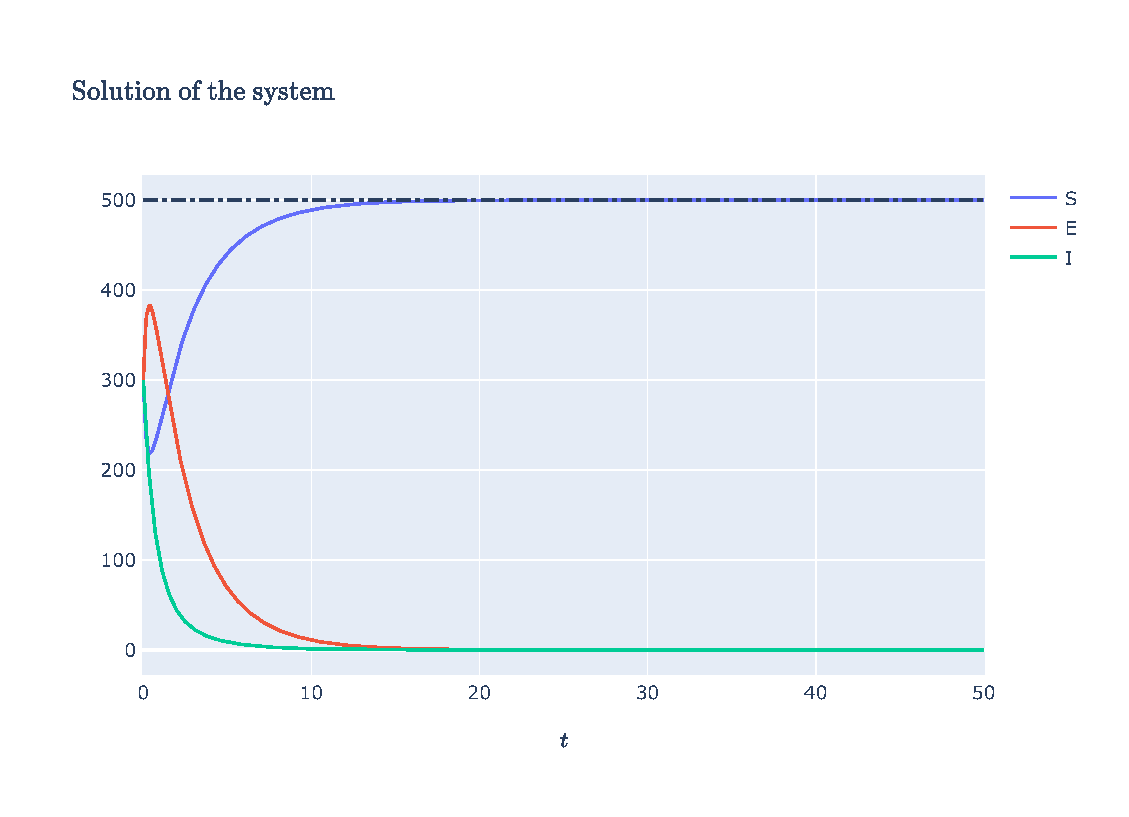
\includegraphics[width=\linewidth]{../figures/numerical_study_R0_lt1_1.eps}  
	  \caption{Solution du syst\`eme au cours du temps}
	  \label{fig:numerical study r0 lt 1 a}
	\end{subfigure}
	\begin{subfigure}{0.49\textwidth}
	  \centering
	  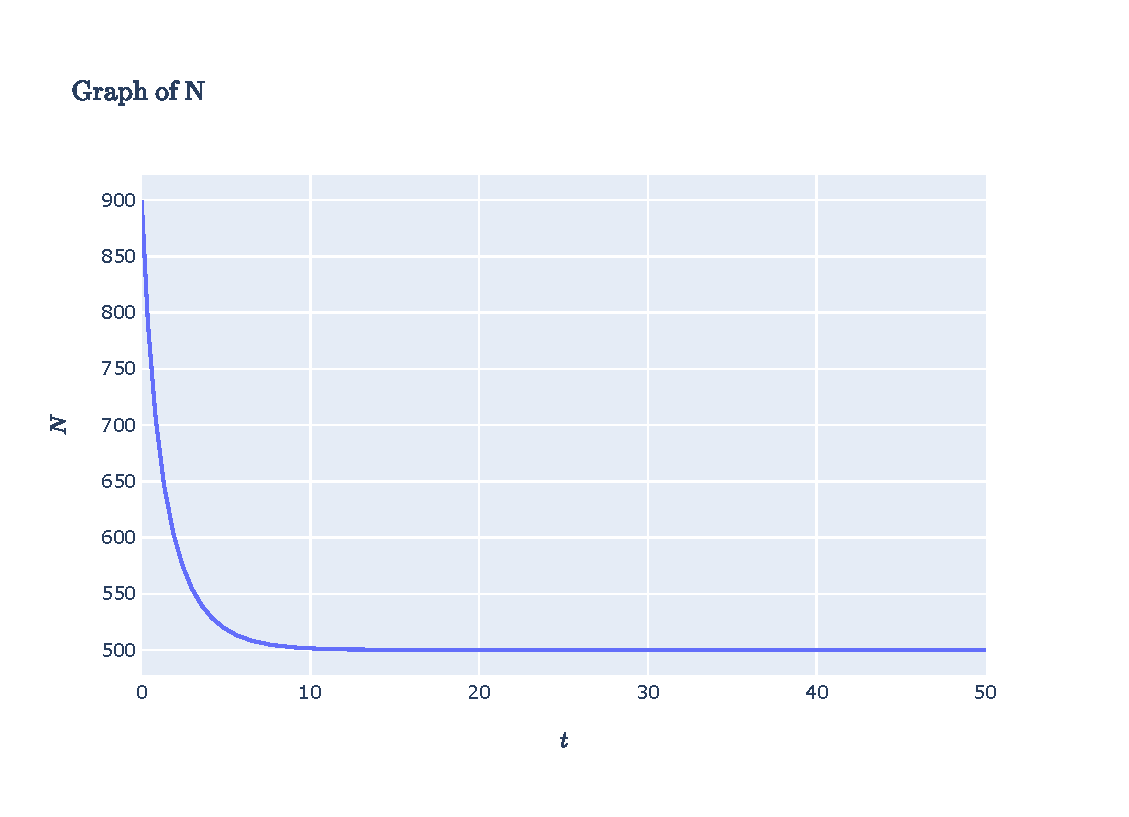
\includegraphics[width=\linewidth]{../figures/numerical_study_R0_lt1_2.eps}  
	  \caption{\'Evolution de la population totale au cours du temps}
	  \label{fig:numerical study r0 lt 1 b}
	\end{subfigure}\\
	\begin{subfigure}{0.49\textwidth}
	  \centering
	  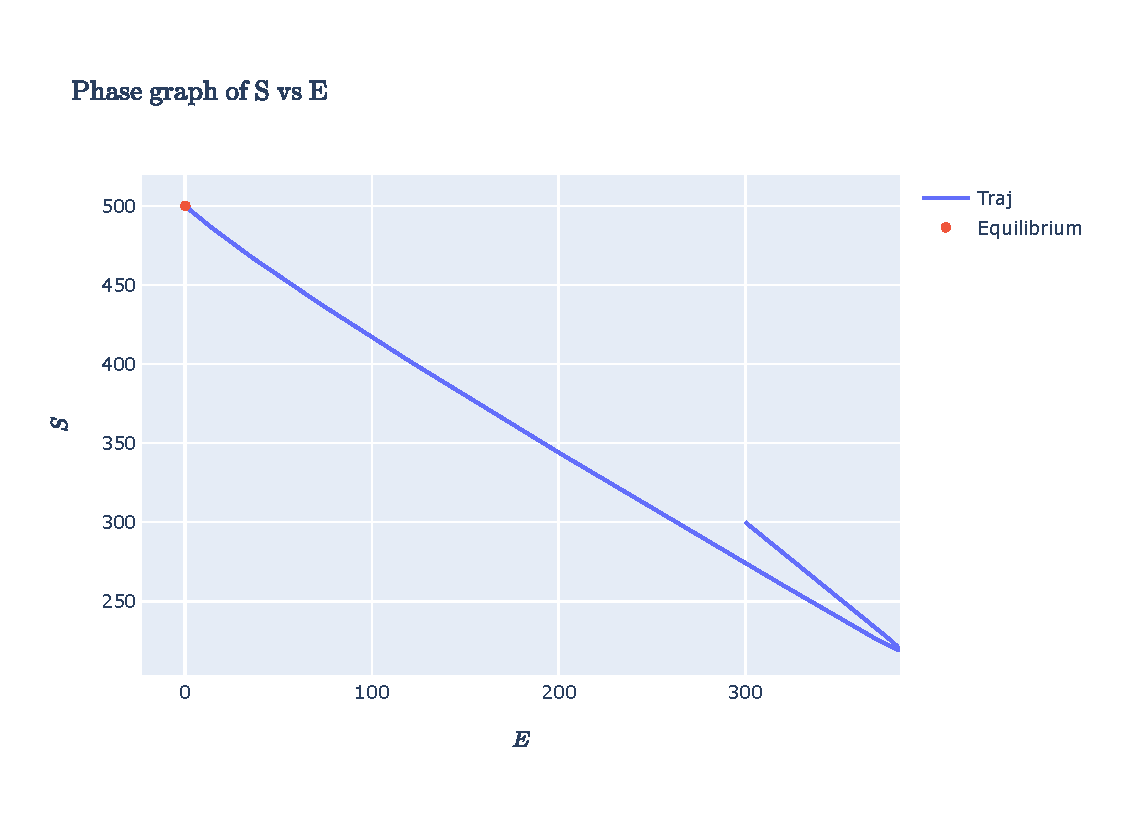
\includegraphics[width=\linewidth]{../figures/numerical_study_R0_lt1_3.eps}  
	  \caption{Portait de phase $S$ en fonction de $E$}
	  \label{fig:numerical study r0 lt 1 c}
	\end{subfigure}
	\begin{subfigure}{0.49\textwidth}
	  \centering
	  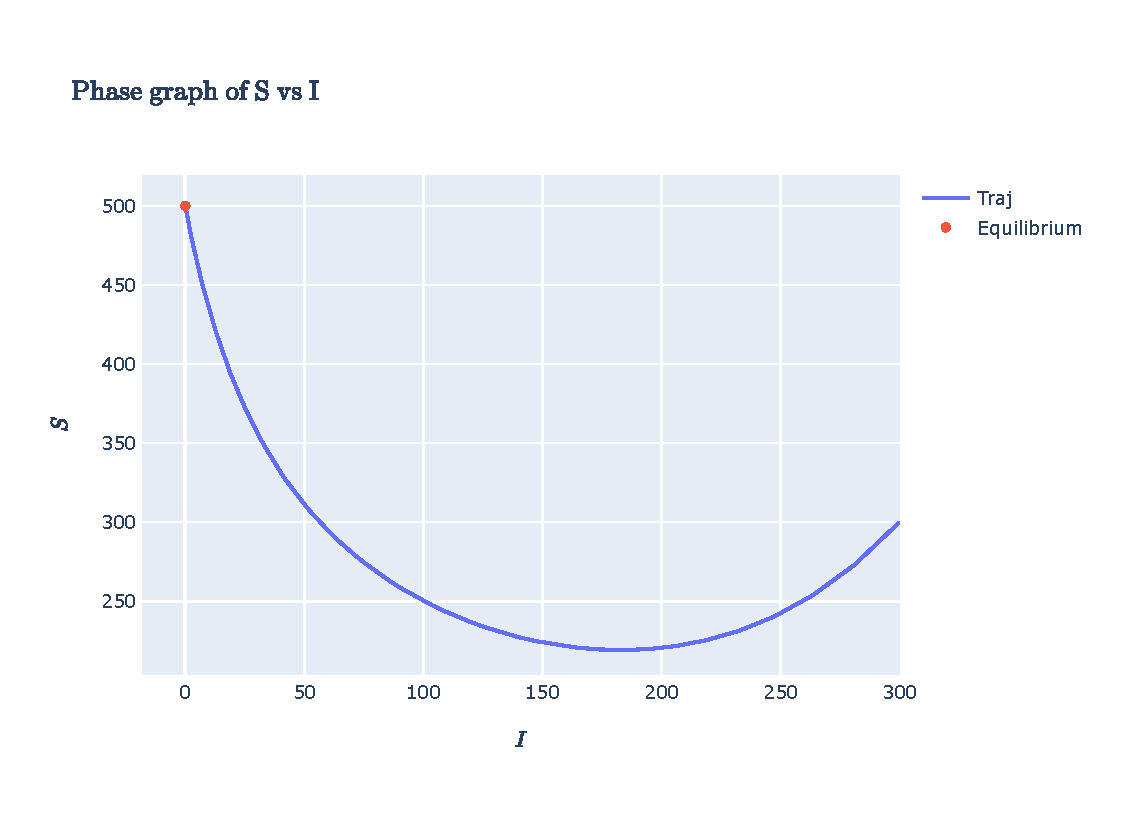
\includegraphics[width=\linewidth]{../figures/numerical_study_R0_lt1_4.eps}  
	  \caption{Portait de phase $S$ en fonction de $I$}
	  \label{fig:numerical study r0 lt 1 d}
	\end{subfigure}
	\centering
	\caption{\'Etude num\'erique du syst\`eme pour $R_0 < 1$, $S_0 = 300, E_0 = 300, I_0 = 300$ \\
	$b =0.5, a = 1, \sigma = \frac{1}{13}, \alpha = \frac{1}{73}, \beta = \frac{1}{79.69}$ et $\gamma = \frac{1}{10000}$
	}
	\label{fig:numerical study r0 lt 1}
\end{figure}
\paragraph{}
Sur la Figure \ref{fig:numerical study r0 lt 1} on repr\'esent\'e la trajectoire et diff\'erents portraits de phases pour $S_0 = 300, E_0 = 300, I_0 = 300, b =0.5, a = 1, \sigma = \frac{1}{13}, \alpha = \frac{1}{73}, \beta = \frac{1}{79.69}$ et $\gamma = \frac{1}{10000}$ ce qui donne $R_0 \approx 0.44$. 

Comme $R_0 < 1$ on s'attend \`a atteindre le DFE (repr\'esent\'e par la ligne en pointill\'es sur la Figure \ref{fig:numerical study r0 lt 1 a}). En effet on peut voir sur la Figure \ref{fig:numerical study r0 lt 1 a} que le nombre d'individus susceptibles est croissant et tend vers $K$. On observe \'egalement que le nombre d'infect\'es est strictement d\'ecroissant, alors que que le nombre d'expos\'es croit l\'eg\'erement avnt de commencer \`a d\'ecroitre (Cela se voit aussi sur la Figure \ref{fig:numerical study r0 lt 1 c}). 

Sur la figure \ref{fig:numerical study r0 lt 1 b} on observe que la population totale d\'ecroit ce qui est normal car le nombre initial  d'individus infect\'es et expos\'es \'etait \'elev\'e par rapport \`a la capacit\'e du milieu.



\begin{figure}[th]
	\begin{subfigure}{0.49\textwidth}
	  \centering
	  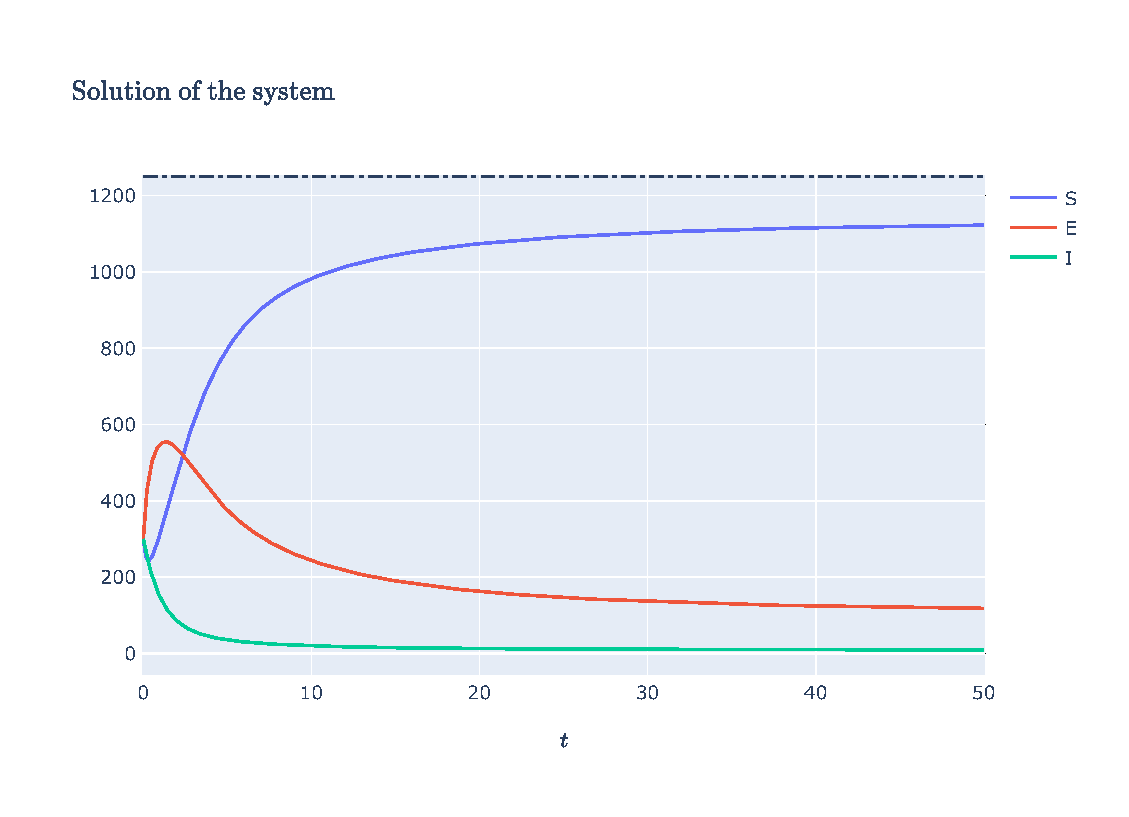
\includegraphics[width=\linewidth]{../figures/numerical_study_R0_gt1_1.eps}  
	  \caption{Solution du syst\`eme au cours du temps}
	  \label{fig:numerical study r0 gt 1 a}
	\end{subfigure}
	\begin{subfigure}{0.49\textwidth}
	  \centering
	  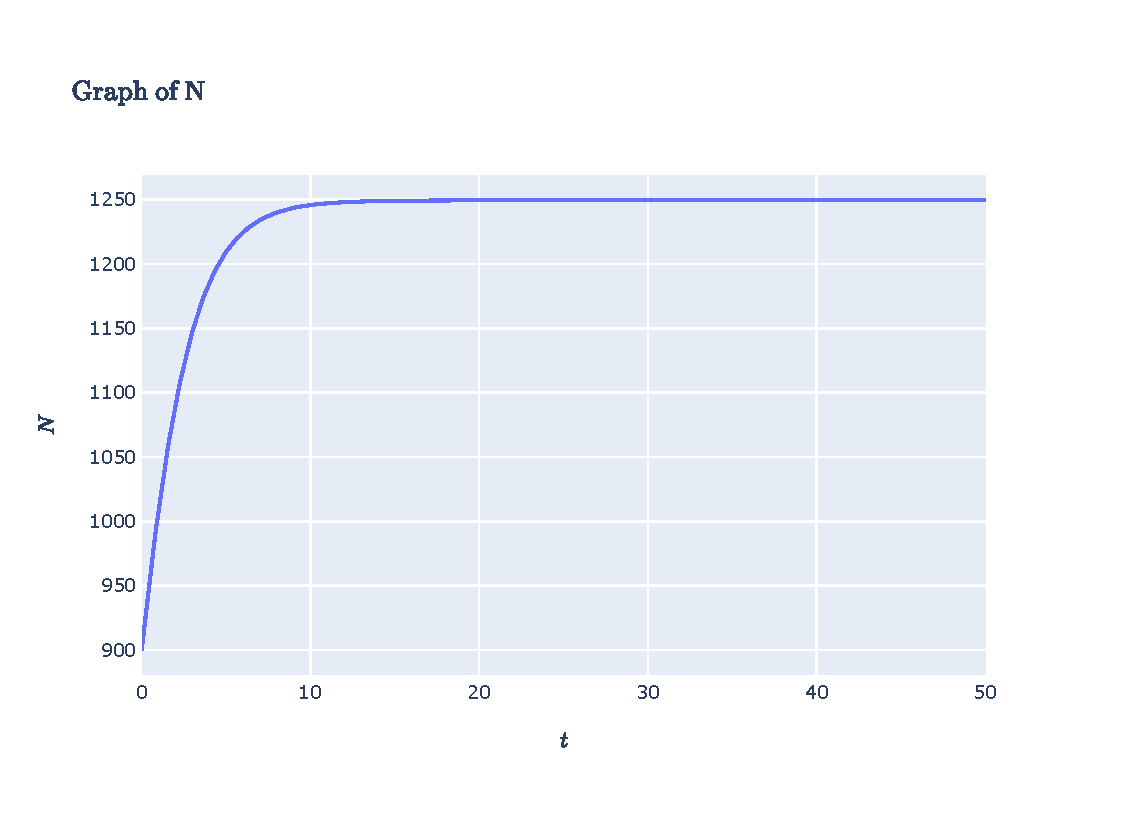
\includegraphics[width=\linewidth]{../figures/numerical_study_R0_gt1_2.eps}  
	  \caption{\'Evolution de la population totale au cours du temps}
	  \label{fig:numerical study r0 gt 1 b}
	\end{subfigure}\\
	\begin{subfigure}{0.49\textwidth}
	  \centering
	  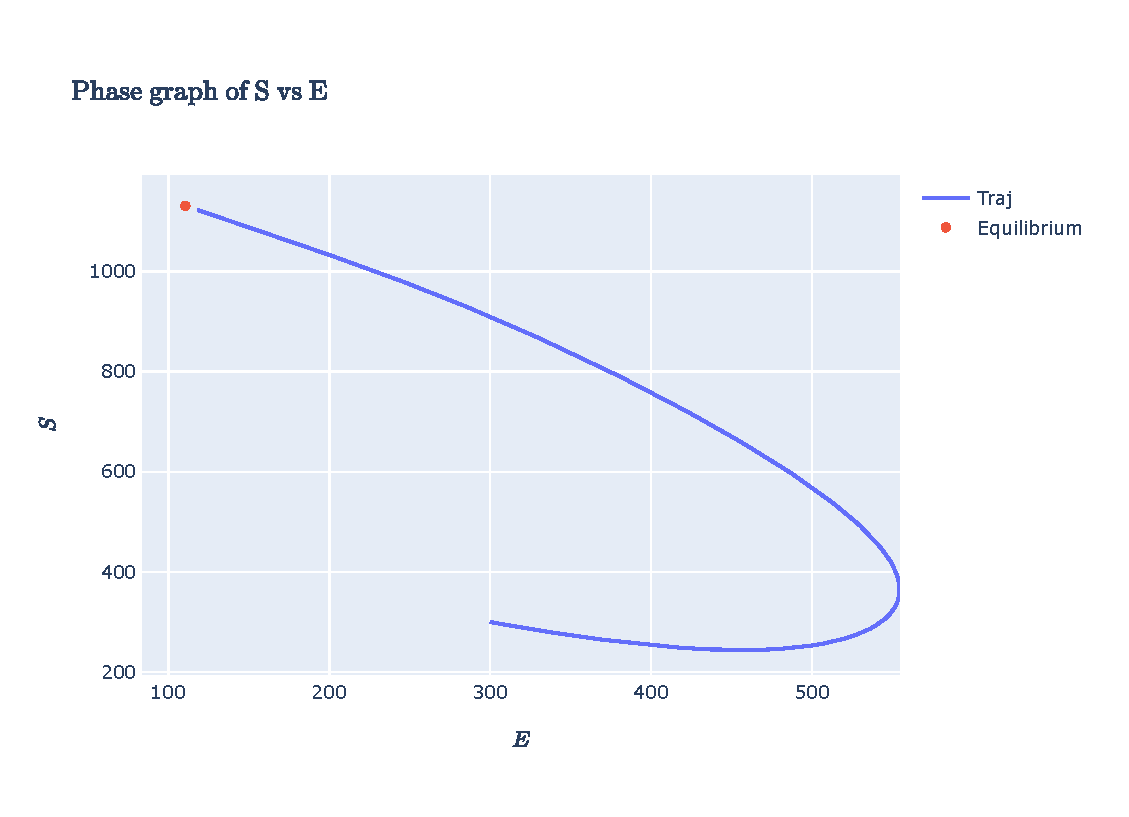
\includegraphics[width=\linewidth]{../figures/numerical_study_R0_gt1_3.eps}  
	  \caption{Portait de phase $S$ en fonction de $E$}
	  \label{fig:numerical study r0 gt 1 c}
	\end{subfigure}
	\begin{subfigure}{0.49\textwidth}
	  \centering
	  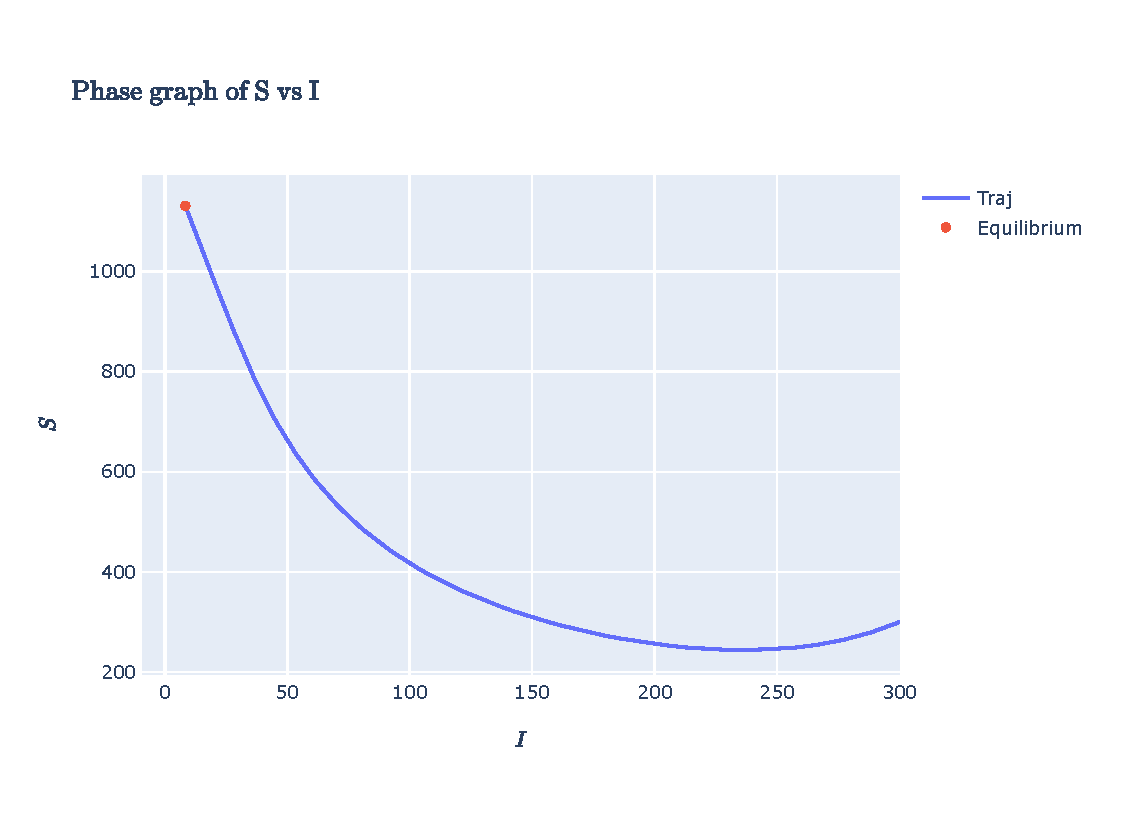
\includegraphics[width=\linewidth]{../figures/numerical_study_R0_gt1_4.eps}  
	  \caption{Portait de phase $S$ en fonction de $I$}
	  \label{fig:numerical study r0 gt 1 d}
	\end{subfigure}
	\centering
	\caption{\'Etude num\'erique du syst\`eme pour $R_0 > 1$, $S_0 = 300, E_0 = 300, I_0 = 300$ \\
	$b =0.5, a = 1, \sigma = \frac{1}{13}, \alpha = \frac{1}{73}, \beta = \frac{1}{79.69}$ et $\gamma = \frac{1}{2500}$
	}
	\label{fig:numerical study r0 gt 1}
\end{figure}
\paragraph{}
Sur la Figure \ref{fig:numerical study r0 gt 1}, on a effectu\'e la m\^eme \'etude pour $S_0 = 300, E_0 = 300, I_0 = 300, b =0.5, a = 1, \sigma = \frac{1}{13}, \alpha = \frac{1}{73}, \beta = \frac{1}{79.69}$ et $\gamma = \frac{1}{2500}$ ($R_0 \approx 1.11$). 

Cette fois-ci, on s'attend \`a ce que les trajectoires soient attir\'ees par l'\'equilibre end\'emique. C'est effectivement ce aue l'on observe sur les figures \ref{fig:numerical study r0 gt 1 c} et \ref{fig:numerical study r0 gt 1 d}. La trajectoire est de fait tr\`es proche de celle de la Figure \ref{fig:numerical study r0 lt 1}, except\'e que le syst\`eme se stabilise dans un \'etat non nul pour $E$ et $S$.

 On remarque aussi que cette fois, comme la population intiale \'etait tr\`es inf\'erieure \`a la capacit\'e du milieu, la populaion totale augmente au cours du temps.


\section{Mod\`ele de vaccination}
On \'etudie maintenant le  mod\`ele SI avec vaccination dont le sch\'ema est pr\'esent\'e \`a la Figure \ref{fig:schema ex 2}:
\[
\left\{ \begin{aligned}
\dt S &= (1-p) \pi - \mu S -\beta I + \beta_v I_v) S\\
\dt {S_v} &= p\pi - \mu S_v- (1-r ) (\beta I + \beta_v I_v)S_v \\
\dt I &= (\beta I + \beta_v I_v)S - (\mu + \nu) I\\
\dt{ I_v} &= (1-r)(\beta I+ \beta_v I_v)S_v - (\mu + \nu_v)I_v
\end{aligned}
\right.
\]
\begin{figure}
	\centering
	\includegraphics{shema ex 2.eps}
	\caption{Sch\'ema du mod\`ele de vaccination}
	\label{fig:schema ex 2}
\end{figure}

\subsection{Interpretation du mod\`ele}
Les parametres du mod\`ele peuvent s'interpreter de la façon suivante :
\begin{itemize}
	\item[$\pi$] Croissance fixe de la population
	\item[$p$] taux de vaccination des nouveaux-n\'es
	\item[$\mu$] taux de mortalit\'e dans la population (hors maladie)
	\item[$\beta$] taux de transmission lors d'un contact entre un individu infect\'e non vaccin\'e et un individu suceptible
	\item[$\beta_v$] taux de transmission lors d'un contact entre un individu infect\'e vaccin\'e et un individu suceptible
	\item[$r$] taux de r\'esistance \`a la contamination des individus vaccin\'es
	\item[$\nu$] taux de mortalit\'e li\'e \`a la maladie dans la population non vaccin\'ee 
	\item[$\nu_v$] taux de mortalit\'e li\'e \`a la maladie dans la population vaccin\'ee 
\end{itemize}

\subsection{\'Equilibre sain}
On cherche un \'equilibre sain, c'est-\`a-dire un point $(\tilde S, \tilde S_v, \tilde I, \tilde I_v )$ tel que,
\[
\left\{\begin{aligned}
\dt {\tilde S} &= 0\\ 
\dt {\tilde S_v} &= 0\\
\tilde I &= 0\\
\tilde I_v &= 0
\end{aligned}
\right.
\]

On a donc
\begin{align*}
	&\left\{
	\begin{aligned}
		0 = (1-p) \pi - \mu \tilde S\\
		0 = p\pi - \mu \tilde S_v
	\end{aligned}
	\right.\\
	\ssi & \left\{ 
	\begin{aligned}
		\tilde S = \frac{(1-p) \pi}{\mu }\\
		\tilde S_v = \frac{p\pi}{ \mu }
	\end{aligned}\right.
\end{align*}


\subsection{Calcul du $R_0$}
On cherche ensuite \`a calculer le taux de reproduction de base ($R_0$). Pour cela on commence par r\'e\'ecrire le syst\`eme sous forme matricielle. On cherche donc $M_1(S,S_v,I,I_v)$ telle que,
\[
\begin{pmatrix}
\dt S\\
\dt {S_v} 
\end{pmatrix} =
M \cdot \begin{pmatrix}
S - \tilde S\\
S_v - \tilde S_v\\
I\\
I_v
\end{pmatrix}
\]

Or, on a
\begin{align*}
\dt S &= (1-p)\pi -\mu S - (\beta I + \beta_v I_v)S\\
&=  (1-p) \pi - \mu \left(S -(1-p)\frac{\pi}{\mu}\right)+ \mu (1-p)\frac{\pi}{\mu}- \beta SI - \beta_v S I_v\\
&= - \mu \left(S -(1-p)\frac{\pi}{\mu}\right)- \beta SI - \beta_v S I_v\\
\intertext{Et}
\dt {S_v} &= P \pi - \mu S_v - (1-r)(\beta I + \beta_v I_v)S_v\\
&= p \pi - \mu \left(S_v - p \frac{\pi}{\mu}\right) + \mu p \frac{\pi}{\mu} - (1-r)(\beta I - \beta_v I_v)S_v\\
&= - \mu \left(S_v - p \frac{\pi}{\mu}\right)  - (1-r)(\beta I - \beta_v I_v)S_v\\
\intertext{Donc,}
M_1 &= \begin{pmatrix}
-\mu & 0 & -\beta S & - \beta_v S\\
0 & -\mu & -(1-r) \beta S_v & -(1-r) \beta_v S_v
\end{pmatrix}
\end{align*}

On pose de plus, $M_1 = [M_{11}, M_{12}]$ avec :
\[M_1 = \begin{pmatrix}
-\mu & 0 \\
0 & -\mu 
\end{pmatrix}
\quad \text{et} \quad 
\begin{pmatrix}
-\beta S & - \beta_v S\\
(1-r) \beta S_v & -(1-r) \beta_v S_v
\end{pmatrix}
\]


On cherche \'egalement $M{22}$ telle que,
 \[
\begin{pmatrix}
\dt I\\
\dt {I_v} 
\end{pmatrix} =
M_{22} \cdot \begin{pmatrix}
I\\
I_v
\end{pmatrix}
\]
 Or comme,
 \begin{align*}
 	\dt I &= (\beta I + \beta_v I_v)S - (\mu + \nu) I\\
 		&= (\beta  S - \mu - \nu ) I + \beta_v S I_v\\
 	\intertext{et}
 	\dt {I_v} &= (1-r)(\beta I+ \beta_vI_v)S_v - (\mu + \nu_v)I_v\\
 		&= ((1-r)\beta_v S_v - \mu - \nu_v )I_v + (1-r)\beta S_v I\\
 	\intertext{on a :}
 	M_{22} &=  \begin{pmatrix}
		\beta S - \mu - \nu  & \beta_v S\\
 		(1-r)\beta S_v & (1-r)\beta_v S_v - \mu - \nu_v 
	\end{pmatrix}
 \end{align*}

On peut r\'e\'ecrire cette matrice sous la forme $F + V$ en posant :
 \begin{align*}
 	F &= \begin{pmatrix}
		\beta S  & \beta_v S\\
 		(1-r)\beta S_v & (1-r)\beta_v S_v 
	\end{pmatrix}\\
	V &= \begin{pmatrix}
		- \mu - \nu  & 0\\
 		0 &  - \mu - \nu_v 
	\end{pmatrix}
 \end{align*}
On obtient alors une d\'ecomposition r\'eguli\`ere, avec  $F$ positive et $V$ de Metzler. Par d\'efinition le taux de reproduction de base est alors (les matrices \'etant prises en $(\tilde S, \tilde {S_v})$:
\[
R_0 = \rho (-F V^{-1})
\]


De plus, 
\begin{align*}
	\det V &= (- \mu -\nu)(-\mu-\nu_v)\\
	\intertext{donc}
	V^{-1} &= \begin{pmatrix}
		\frac{-\mu-\nu_v}{(-\mu - \nu)(-\mu - \nu_v)} & 0\\
		0 & \frac{-\mu-\nu}{(-\mu - \nu)(-\mu - \nu_v)}
	\end{pmatrix}\\
	&= \begin{pmatrix}
		-\mu-\nu & 0\\
		0 & -\mu-\nu_v
	\end{pmatrix}\\
	\intertext{et, }
	-F V^{-1} &= 
		\begin{pmatrix}
			\frac{\beta S}{ \mu + \nu} & \frac{\beta_v S}{ \mu + \nu_v} \\
			(1-r)\frac{\beta S_v}{ \mu + \nu}  & (1-r)\frac{\beta_v S_v}{ \mu + \nu_v} 
		\end{pmatrix} \\
	\intertext{D'o\`u}
	\det(-FV^{-1} - \lambda I) &= \left(\frac{\beta S}{ \mu + \nu} - \lambda \right) \left((1-r)\frac{\beta_v S_v}{ \mu + \nu_v} -\lambda \right) - (1-r)\frac{\beta S_v}{ \mu + \nu}\frac{\beta_v S}{ \mu + \nu_v}
\end{align*}
Les valeurs propres de $-F V^{-1}$ sont donc les solutions de l'\'equation :
\begin{align*}
	&& 0 &= \left(\frac{\beta S}{ \mu + \nu} - \lambda \right) \left((1-r)\frac{\beta_v S_v}{ \mu + \nu_v} -\lambda \right) - (1-r)\frac{\beta S_v}{ \mu + \nu}\frac{\beta_v S}{ \mu + \nu_v}\\
	&& &= \frac{\left(\beta S - (\mu +\nu) \lambda\right)\left((1-r)\beta_v S_v- (\mu + \nu_v)\lambda \right) - (1-r) \beta_v S \beta S_v}{(\mu + \nu)(\mu + \nu_v)}\\
	&\ssi& 0 &=  \left(\beta S - (\mu +\nu) \lambda\right)\left((1-r)\beta_v S_v- (\mu + \nu_v)\lambda \right) - (1-r) \beta_v S \beta S_v\\
	&&& = (1-r) \beta_v S \beta S_v - \beta S (\mu + \nu_v) \lambda  - (\mu + \nu)\beta_v S_v \lambda +(\mu + \nu) (\mu + \nu_v) \lambda ^2 - (1-r) \beta_v S \beta S_v\\
	&&& = (\mu + \nu) (\mu + \nu_v) \lambda ^2 - (\beta S (\mu + \nu_v)+ (\mu + \nu)\beta_v S_v) \lambda\\
	&&& = \lambda ((\mu + \nu) (\mu + \nu_v) \lambda  - (\beta S (\mu + \nu_v)+ (\mu + \nu)\beta_v S_v))\\
	&\ssi&& \left\{\begin{aligned}
		\lambda &= 0 \\
		\text{ou } \lambda &= \frac{(\beta S (\mu + \nu_v)+ (\mu + \nu)\beta_v S_v)}{(\mu + \nu) (\mu + \nu_v) \lambda}\\
			&= \frac{\beta S}{\mu + \nu} + \frac{(1-r) \beta_v S_v}{\mu +\nu_v}
	\end{aligned}\right.
\end{align*} 

On a donc, puisque la valeur propre non nulle est toujours positive que, 
\begin{align*}
R_0 &= \frac{\beta \tilde S}{\mu + \nu} + \frac{(1-r) \beta_v \tilde{S_v}}{\mu +\nu_v}\\
&= \frac{\pi}{\mu} \left(\frac{(1-p)\beta}{\mu + \nu} + \frac{p(1-r) \beta_v}{\mu +\nu_v}\right)
\end{align*}


\subsection{R\'e\'ecriture de $R_0$}
En posant, 
\begin{align*}
\beta_{uu} &= \beta\\
\beta_{uv} &= \beta_v\\
\beta_{vu} &= (1-r) \beta\\
\beta_{vv} &= (1-r) \beta_v 
\end{align*}
On peut r\'e\'ecrire $R_0$ sous la forme :
\[
R_0 = \frac{\pi}{\mu} \left(\frac{(1-p)\beta_{uu}}{\mu + \nu} + \frac{p \beta_{vv}}{\mu +\nu_v}\right)
\]

Et la condition $R_0 <1$ peut se r\'e\'ecrire :
\begin{align*}
	&\quad\frac{\pi}{\mu} \left(\frac{(1-p)\beta_{uu}}{\mu + \nu} + \frac{p \beta_{vv}}{\mu +\nu_v}\right)  < 1 \\
	\ssi&\quad  \frac{\pi(1-p)\beta_{uu}}{\mu(\mu+\nu)} < \frac{\pi p\beta_{vv}}{\mu(\mu+\nu_v)}\\
	\ssi&\quad\beta_{uu} < \frac{p}{1-p}\frac{\mu+\nu}{\mu+\nu_v}\beta_{vv}\\
	\ssi&\quad\beta_{vv} > \frac{1-p}{p}\frac{\mu+\nu_v}{\mu+\nu}\beta_{uu}
\end{align*}

\subsection{Simulations num\'eriques}
On pr\'esente ici quelques simulations num\'eriques du mod\`ele.
\begin{figure}[hb]
	\begin{subfigure}{0.49\textwidth}
	  \centering
	  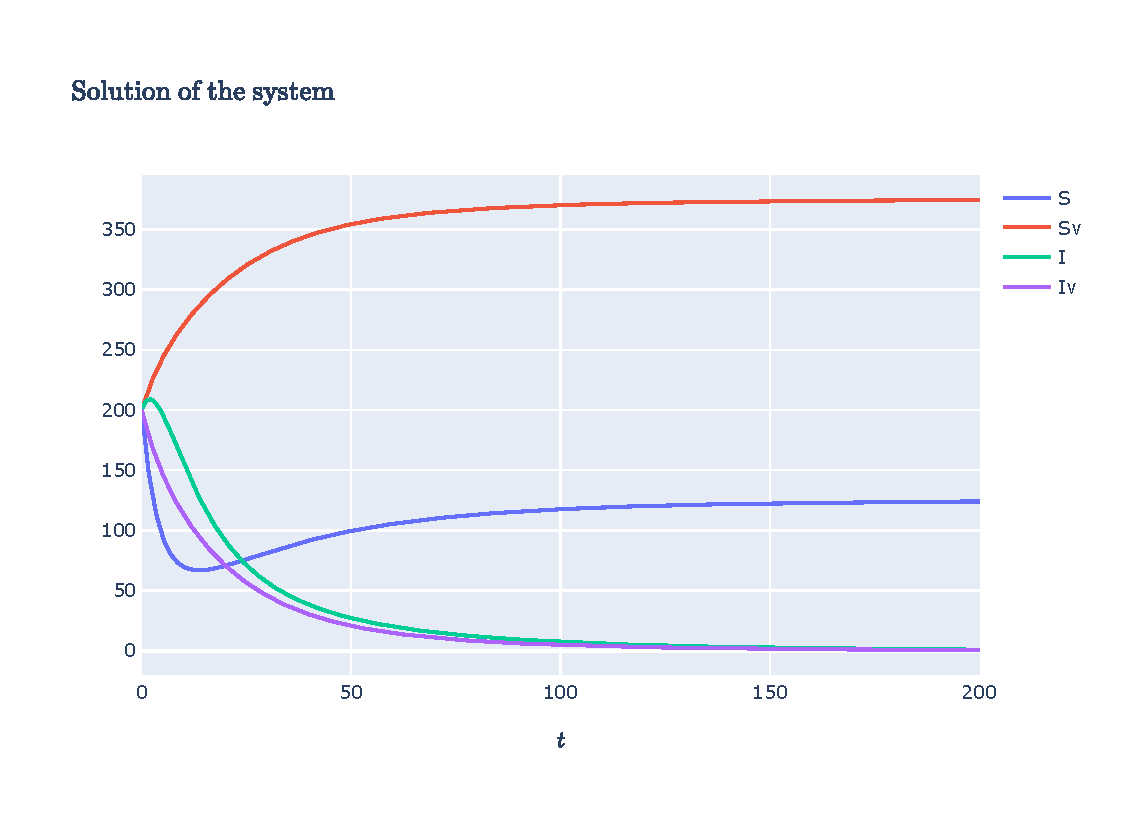
\includegraphics[width=\linewidth]{../figures/ex2_r0_lt_1.eps}  
	  \caption{$p = 3/4,
		r = 8/10, 
		\pi = 50,
		\mu = 1/10$\\
		$\nu = 1/2000,
		\nu_v = 1/4000, R_0 \approx 0.81$}
	  \label{fig:ex2 evolution r0 lt 1}
	\end{subfigure}
	\begin{subfigure}{0.49\textwidth}
	  \centering
	  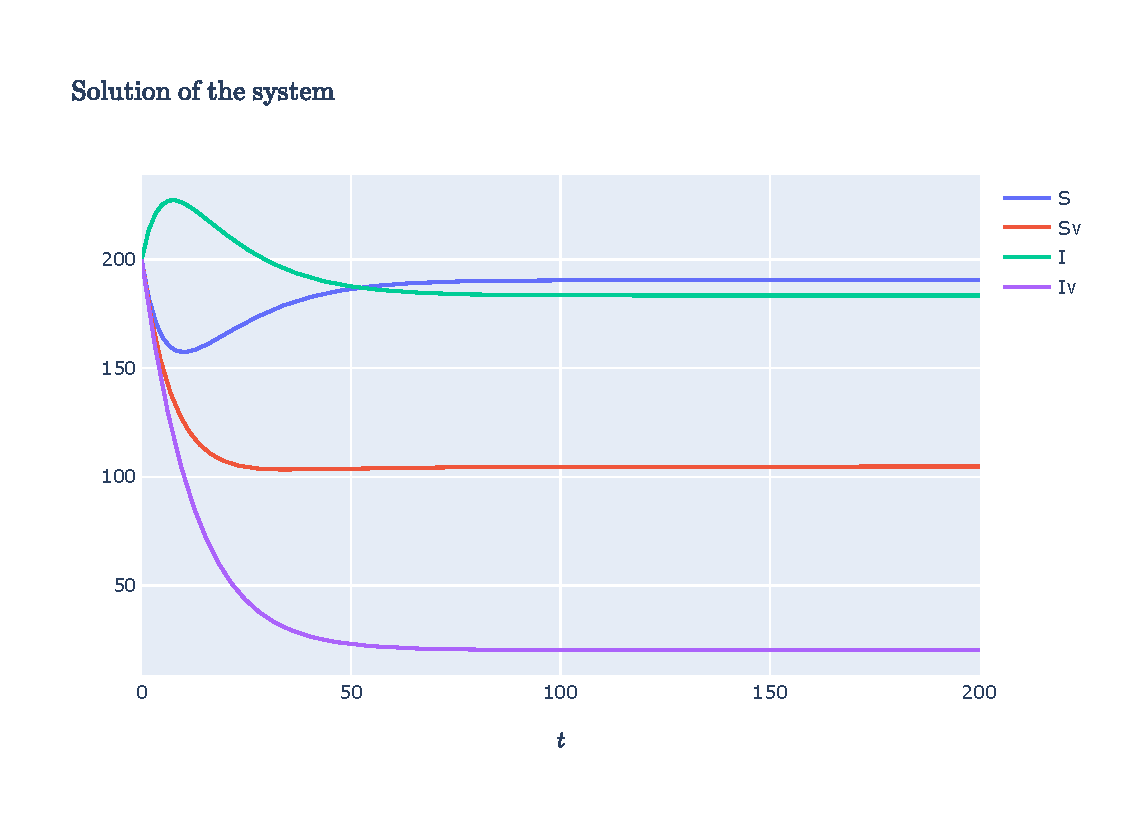
\includegraphics[width=\linewidth]{../figures/ex2_r0_gt_1.eps}  
	  \caption{$p = 1/4,
		r = 8/10, 
		\pi = 50,
		\mu = 1/10$\\
		$\nu = 1/2000,
		\nu_v = 1/4000, R_0 \approx 1.93$}
	  \label{fig:ex2 evolution r0 gt 1}
	\end{subfigure}
	\centering
	\caption{\'Evolution du syst\`eme au cours du temps pour $R_0 < 1$ et $R_0 > 1$
	}
	\label{fig:ex2 evolution}
\end{figure}
\paragraph{} 
La Figure \ref{fig:ex2 evolution} Pr\'esente l'\'evolution en temps du mod\`ele pour deux jeux de param\`etres menant \`a $R_0 < 1$ ou  $R_0 > 1$. Entre ces deux jeux de param\`etres seul le taux de vaccination change ($p = 3/4$ pour la Figure \ref{fig:ex2 evolution r0 lt 1} et $p = 1/4$ pour la Figure \ref{fig:ex2 evolution r0 gt 1}).

 Dans un cas $R_0 <1$ et l'\'epid\'emie s'\'eteint dans l'autre $R_0 >1$ et la maladie est end\'emique. De plus m\^eme dans le cas o\`u $R_0 >1$ les individus vaccin\'es sont moins touch\'es par la maladie que les individus non vaccin\'es. 

Selon ce mod\`ele, la vaccination est un outils majeur dans la pr\'evention et le contr\^ole sde cette \'epid\'emie.


\paragraph{}
La Figure \ref{fig:ex2 IS} pr\'esente l'\'evolution de $I$ en fonction de $S$ ainsi que de $I_v$ en fonction de $S$. La Figure \ref{fig:ex2 SvS} pr\'esente quant \`a elle des portraits de phases $I_v$ en fonction de $I$ et $S_v$ en fonction de $S$ pour diff\'erentes conditions initiales.

\begin{figure}[th]
	\begin{subfigure}{0.49\textwidth}
	  \centering
	  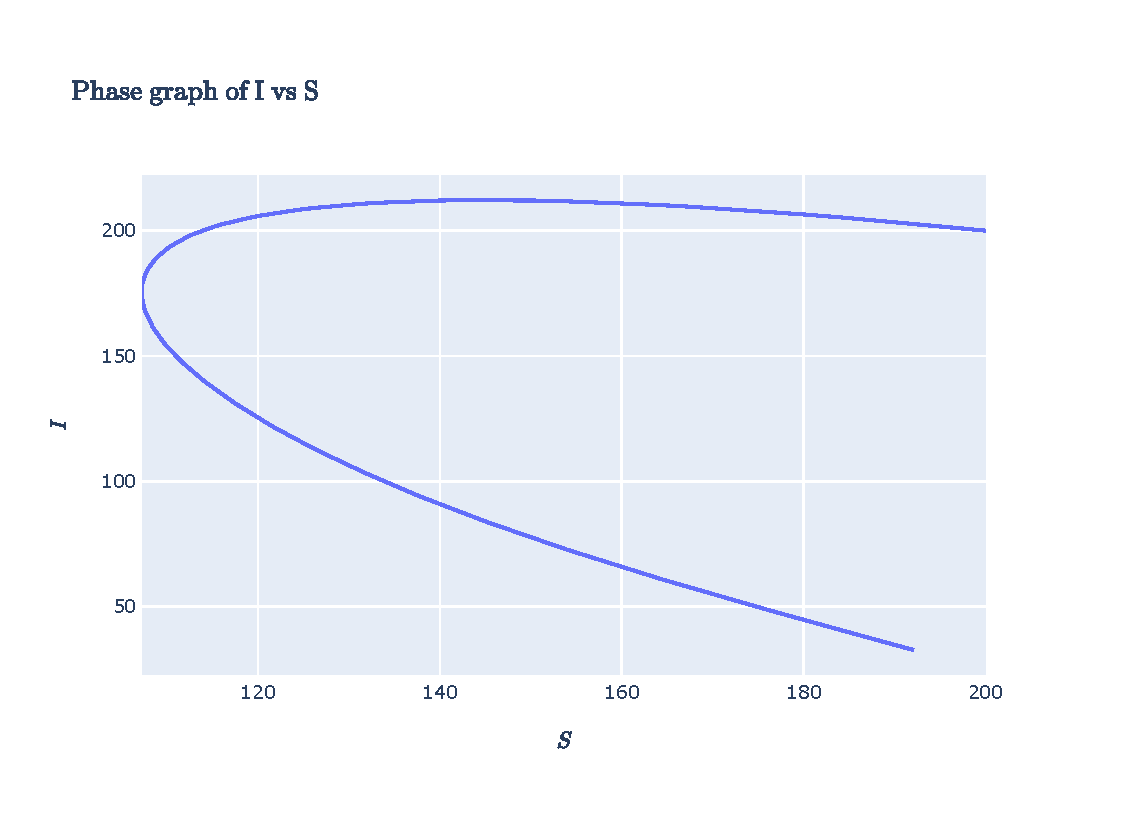
\includegraphics[width=\linewidth]{../figures/ex2_IS_1.eps}  
	  \caption{$p = 1/4,
	  		r = 8/10, 
	  		\pi = 30,
	  		\mu = 1/10 $\\
	  		$\nu = 1/2000,
	  		\nu_v = 1/4000, R_0 \approx 1.16$}
	  
	\end{subfigure}
	\begin{subfigure}{0.49\textwidth}
	  \centering
	  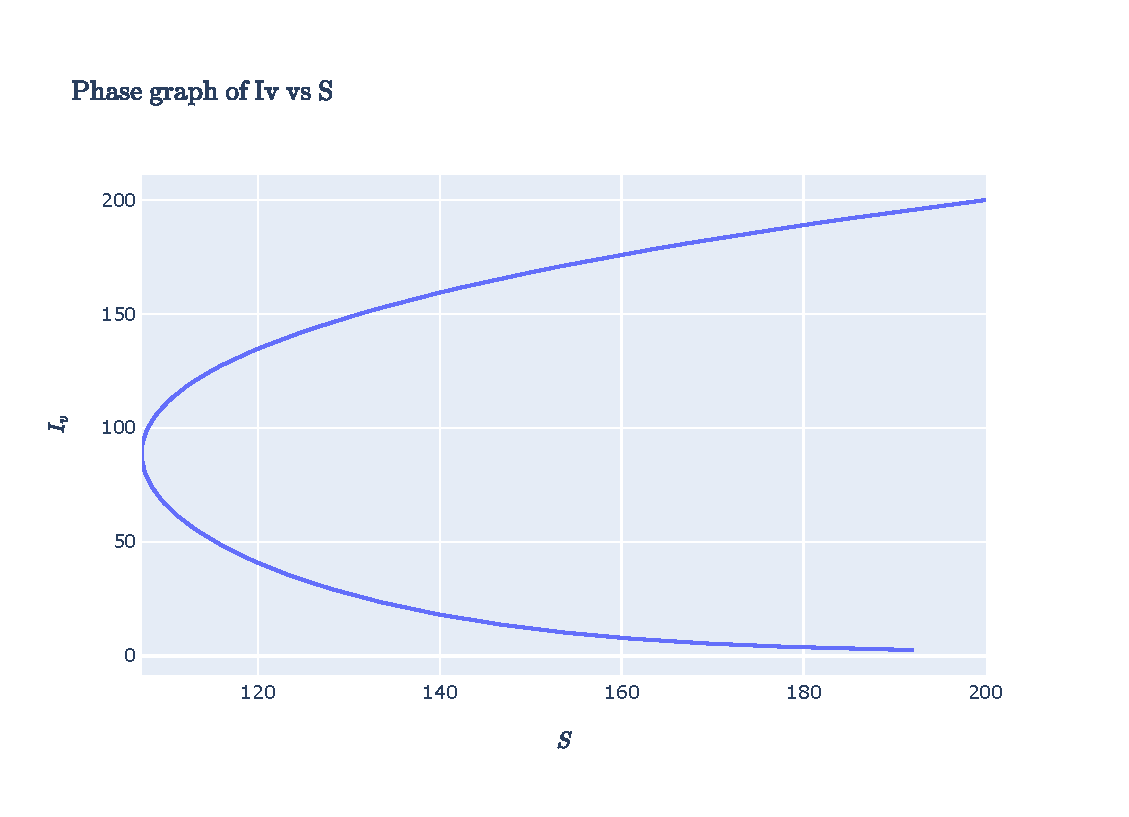
\includegraphics[width=\linewidth]{../figures/ex2_IvS_1.eps}  
	  \caption{$p = 1/4,
	  		r = 8/10, 
	  		\pi = 30,
	  		\mu = 1/10 $\\
	  		$\nu = 1/2000,
	  		\nu_v = 1/4000, R_0 \approx 1.16$}
	\end{subfigure}\\
	\begin{subfigure}{0.49\textwidth}
	  \centering
	  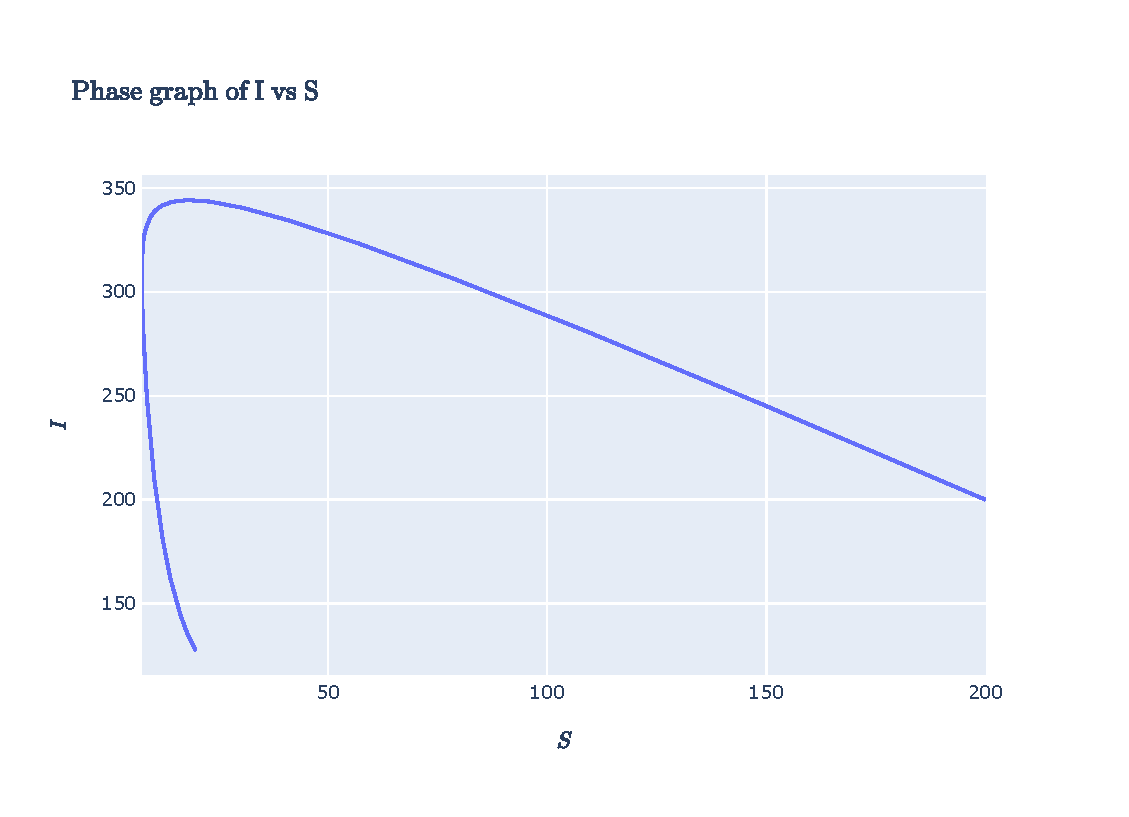
\includegraphics[width=\linewidth]{../figures/ex2_IS_2.eps}  
	  \caption{$p = 1/2,
	  		r = 8/10, 
	  		\pi = 30,
	  		\mu = 1/10$\\$
	  		\nu = 1/500,
	  		\nu_v = 1/200, R_0 \approx 7.26$}
	\end{subfigure}
	\begin{subfigure}{0.49\textwidth}
	  \centering
	  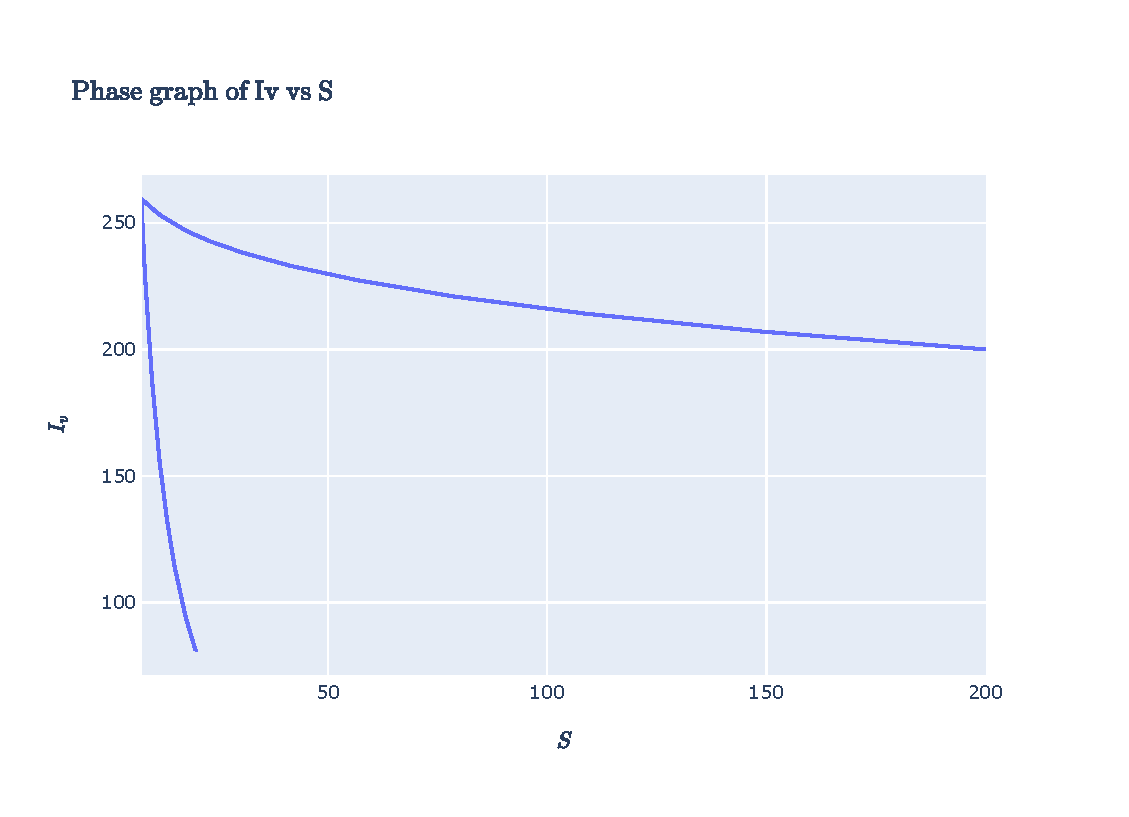
\includegraphics[width=\linewidth]{../figures/ex2_IvS_2.eps}  
	  \caption{$p = 1/4,
	  		r = 8/10, 
	  		\pi = 30,
	  		\mu = 1/10$\\
	  		$\nu = 1/500,
	  		\nu_v = 1/200, R_0 \approx 7.26$}
	\end{subfigure}

	\centering
	\caption{Portraits de Phase $I$ en fonction de $S$ et $I_v$ en fonction de $S$. 
	}
	\label{fig:ex2 IS}
\end{figure}


\begin{figure}[th]
	\begin{subfigure}{0.49\textwidth}
	  \centering
	  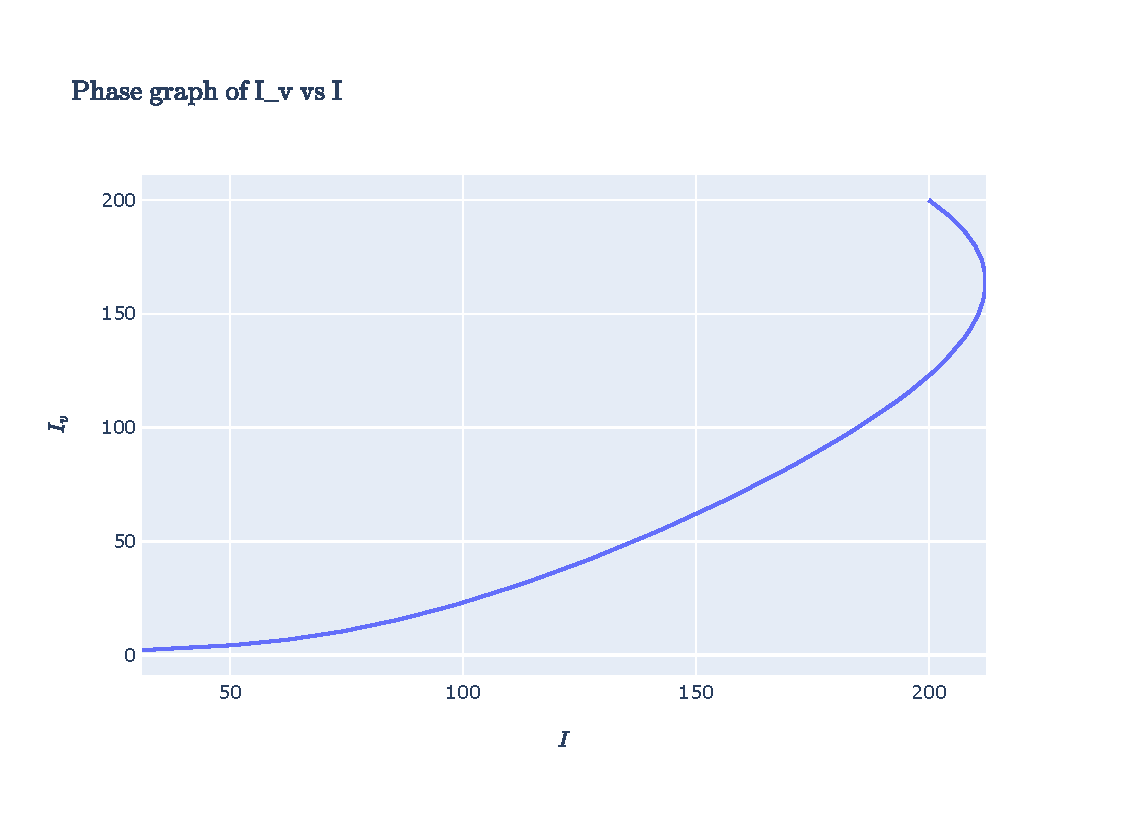
\includegraphics[width=\linewidth]{../figures/ex2_IvI_1.eps}  
	  \caption{$S_0 = 200, S_{v0} = 200,I_0 = 200, I_{v0} = 200$}
	  
	\end{subfigure}
	\begin{subfigure}{0.49\textwidth}
	  \centering
	  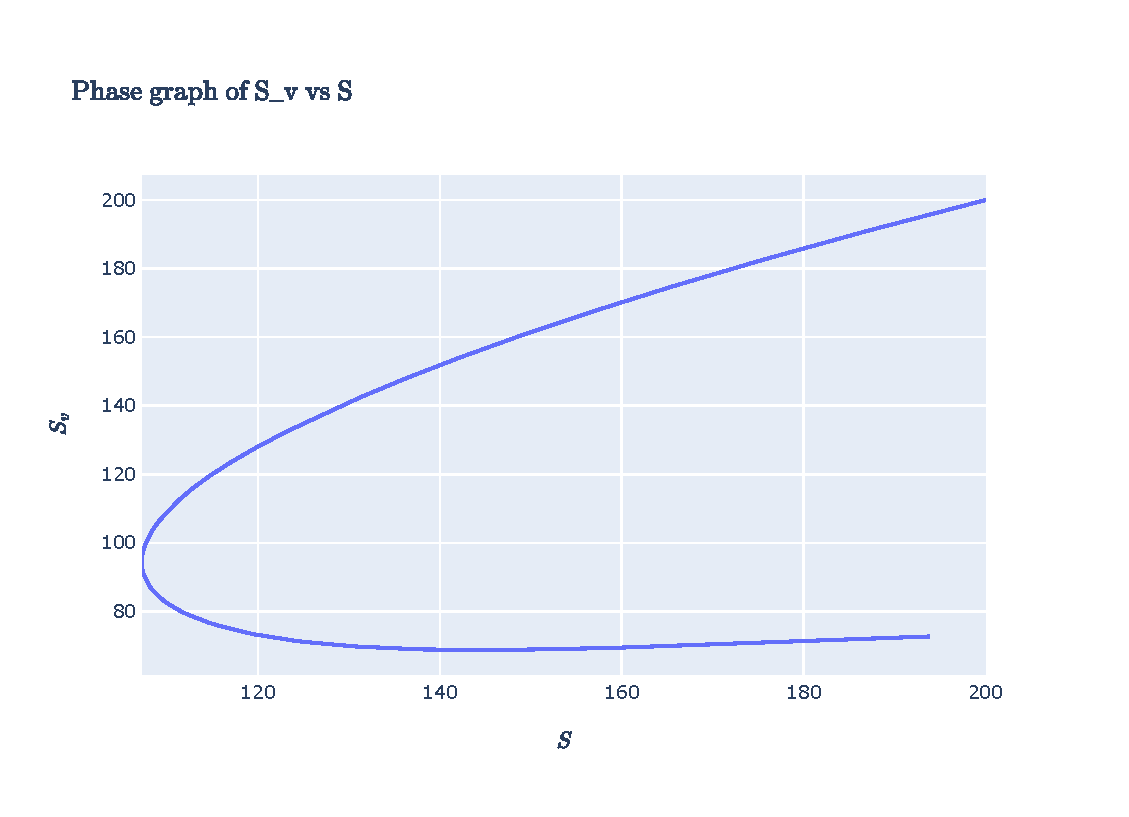
\includegraphics[width=\linewidth]{../figures/ex2_SvS_1.eps}  
	  \caption{$S_0 = 200, S_{v0} = 200,I_0 = 200, I_{v0} = 200$}
	\end{subfigure}\\
	\begin{subfigure}{0.49\textwidth}
	  \centering
	  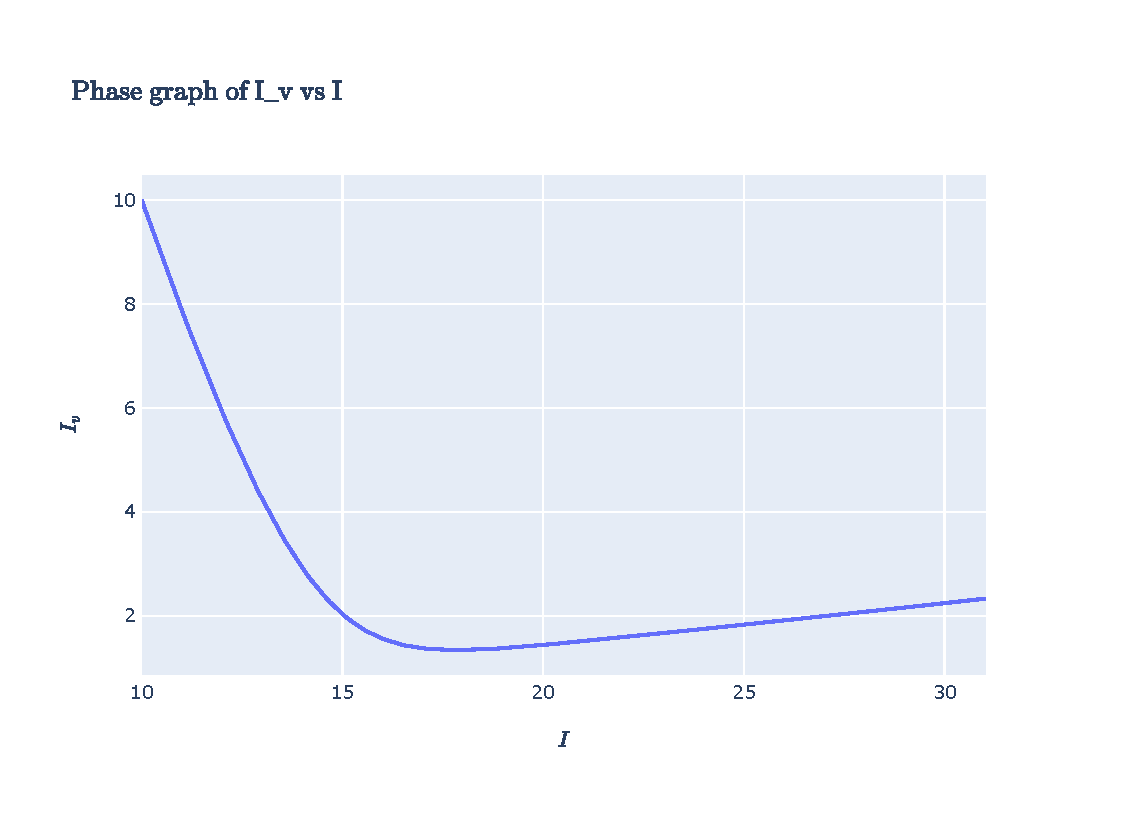
\includegraphics[width=\linewidth]{../figures/ex2_IvI_2.eps}  
	   \caption{$S_0 = 195, S_{v0} = 0,I_0 = 10, I_{v0} = 10$}
	\end{subfigure}
	\begin{subfigure}{0.49\textwidth}
	  \centering
	  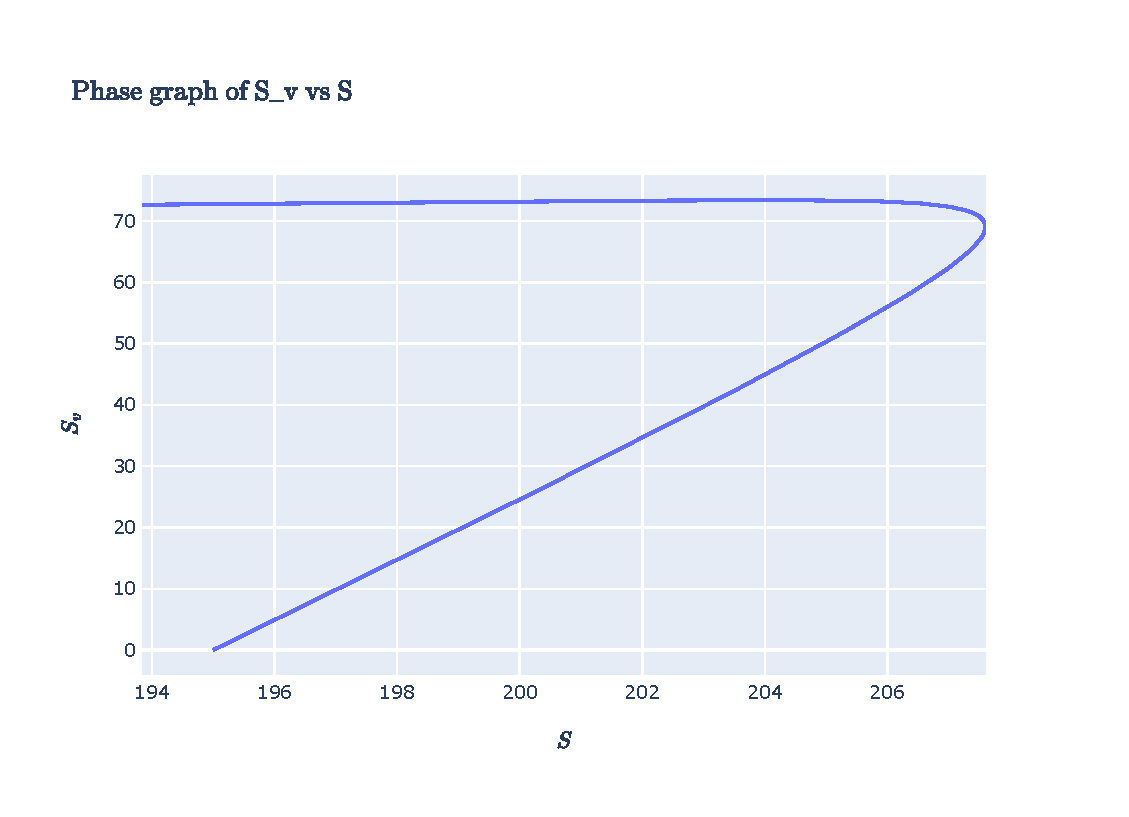
\includegraphics[width=\linewidth]{../figures/ex2_SvS_2.eps}  
	  \caption{$S_0 = 195, S_{v0} = 0,I_0 = 10, I_{v0} = 10$}
	\end{subfigure}\\
	\begin{subfigure}{0.49\textwidth}
	  \centering
	  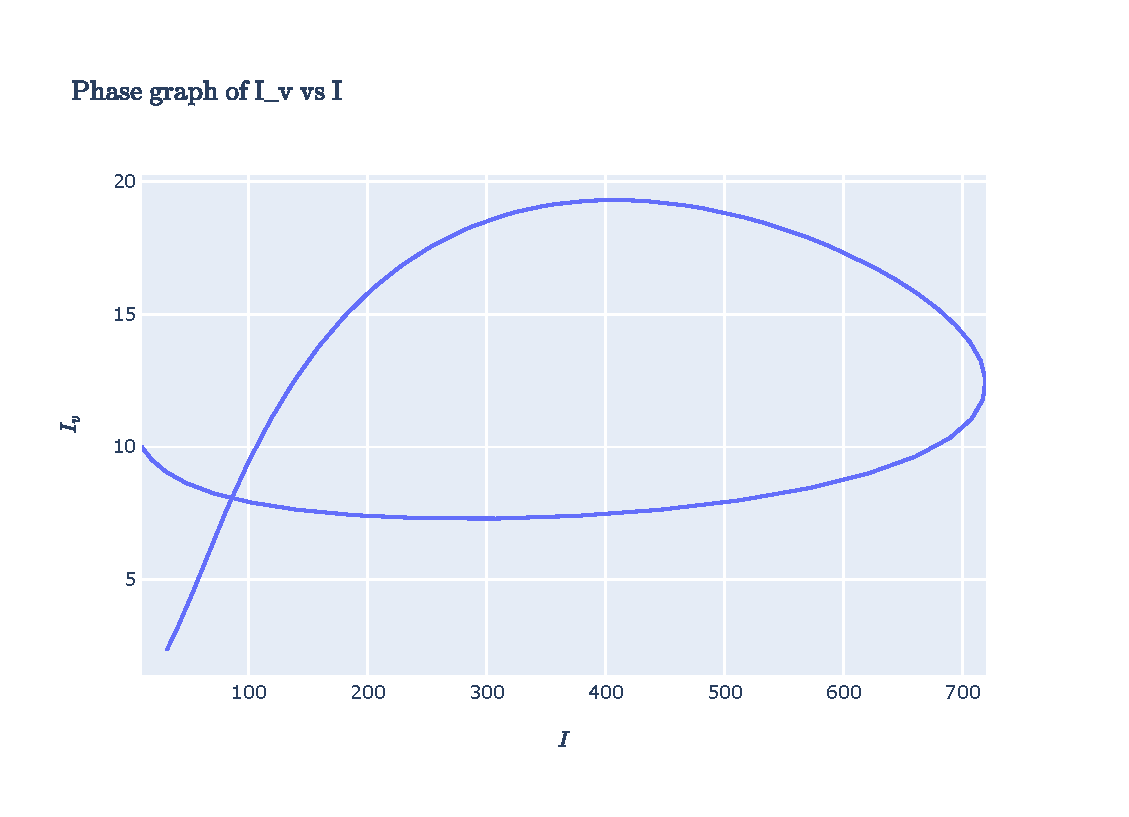
\includegraphics[width=\linewidth]{../figures/ex2_IvI_3.eps}  
	  \caption{$S_0 = 1995, S_{v0} = 0,I_0 = 10, I_{v0} = 10$}
	\end{subfigure}
	\begin{subfigure}{0.49\textwidth}
	  \centering
	  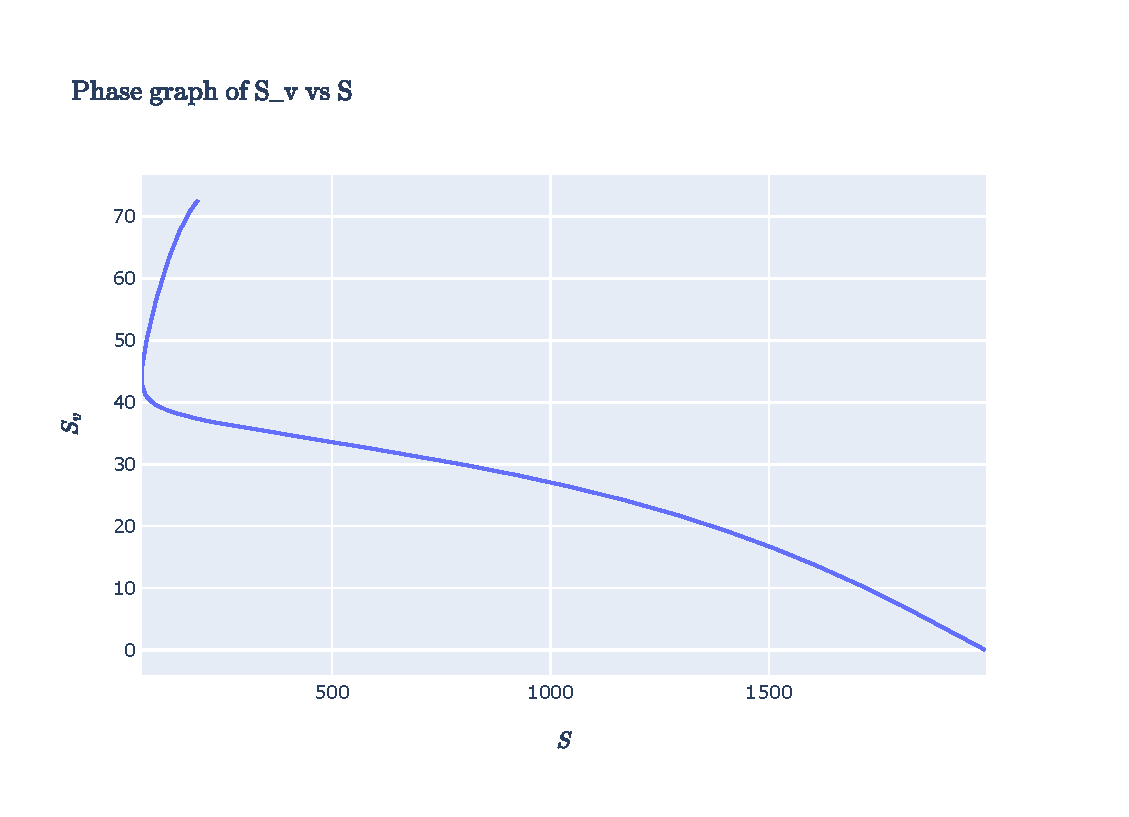
\includegraphics[width=\linewidth]{../figures/ex2_SvS_3.eps}  
	  \caption{$S_0 = 1995, S_{v0} = 0,I_0 = 10, I_{v0} = 10$}
	\end{subfigure}

	\centering
	\caption{Portraits de Phase $I_v$ en fonction de $I$ et $S_v$ en fonction de $S$. \\
	$p = 1/4,
		r = 8/10, 
		\pi = 30,
		\mu = 1/10, \nu = 1/2000,
		\nu_v = 1/4000. R_0 \approx 1.16$ 
	}
	\label{fig:ex2 SvS}
\end{figure}

\clearpage

\section*{Code source}
Les simulations ont \'et\'e r\'ealis\'ees sous python gr\^ace aux biblioth\`eques \texttt{scipy}\footnote{\url{https://www.scipy.org/}} et \texttt{numpy}\footnote{\url{https://numpy.org/}}, les figures ont \'et\'e g\'ener\'ees par la biblioth\`eque \texttt{plotly}\footnote{\url{https://plotly.com/python/}}.

\paragraph{}Un d\'epot contenant le code source utilis\'e pour les simulations ainsi que pour g\'en\'erer ce rapport est disponnible \`a l'adresse \url{https://github.com/celbig/projet_epidemio_m2}.
\end{document}